Pada bagian tatak laksana program yang dibuat akan dijelaskan beberapa langkah-langkah yang dilakukan dalam proses pembuatan program yaitu sebagai berikut.

\subsection{Persiapan lingkungan Pengembangan Aplikasi}
Pengembangan aplikasi presensi \textit{online} akan menggunakan \textit{framework} Laravel. \textit{framework} ini merupakan \textit{framework backend}, namun \textit{framework} ini menyediakan \textit{blade templating} agar dapat mengembangkan sisi \textit{frontend}. \textit{Framework} ini menggunakan konsep MVC (\textit{Model-View-Controller}) yang memisahkan logika aplikasi menjadi tiga bagian utama, sehingga memudahkan pengelolaan dan pengembangan aplikasi dengan lebih terstruktur. Untuk membuat proyek Laravel baru, dibutuhkan PHP dengan versi 8 keatas. Penulis melakukan instalasi XAMPP karena didalamnya sudah termasuk PHP, \textit{apache}, dan basis data MySQL. Instalasi dapat dilakukan melalui tautan \url{https://www.apachefriends.org/download.html}. \textbf{~\ref{fig:tampilan-XAMPP}} menunjukkan tampilan XAMPP setelah selesai instalasi.
 %
    \begin{figure}[!htbp]
    	\centering
    	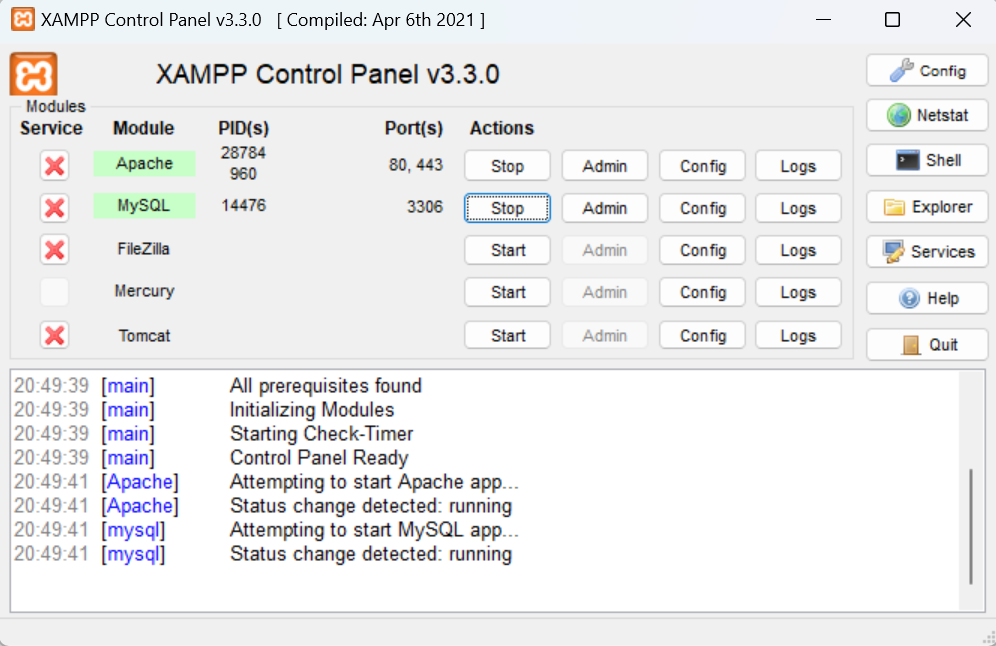
\includegraphics[width=10cm]{Gambar/bab3/start-xampp.png}
    	\caption{Tampilan XAMPP}
    	\label{fig:tampilan-XAMPP}
    \end{figure}
    \FloatBarrier
    %
Setelah itu, dibutuhkan juga Composer untuk \textit{dependency manager} untuk mengelola \textit{package} dan dependensi lainnya. Instalasi Composer dapat dilakukan melalui tautan \url{https://getcomposer.org/download/}. Jika semua sudah ter-\textit{install}, jalankan \textit{command line} yang dapat dilihat pada \textbf{~\ref{fig:command-line-create-laravel}}. 
%
    \begin{figure}[!htbp]
    	\centering
    	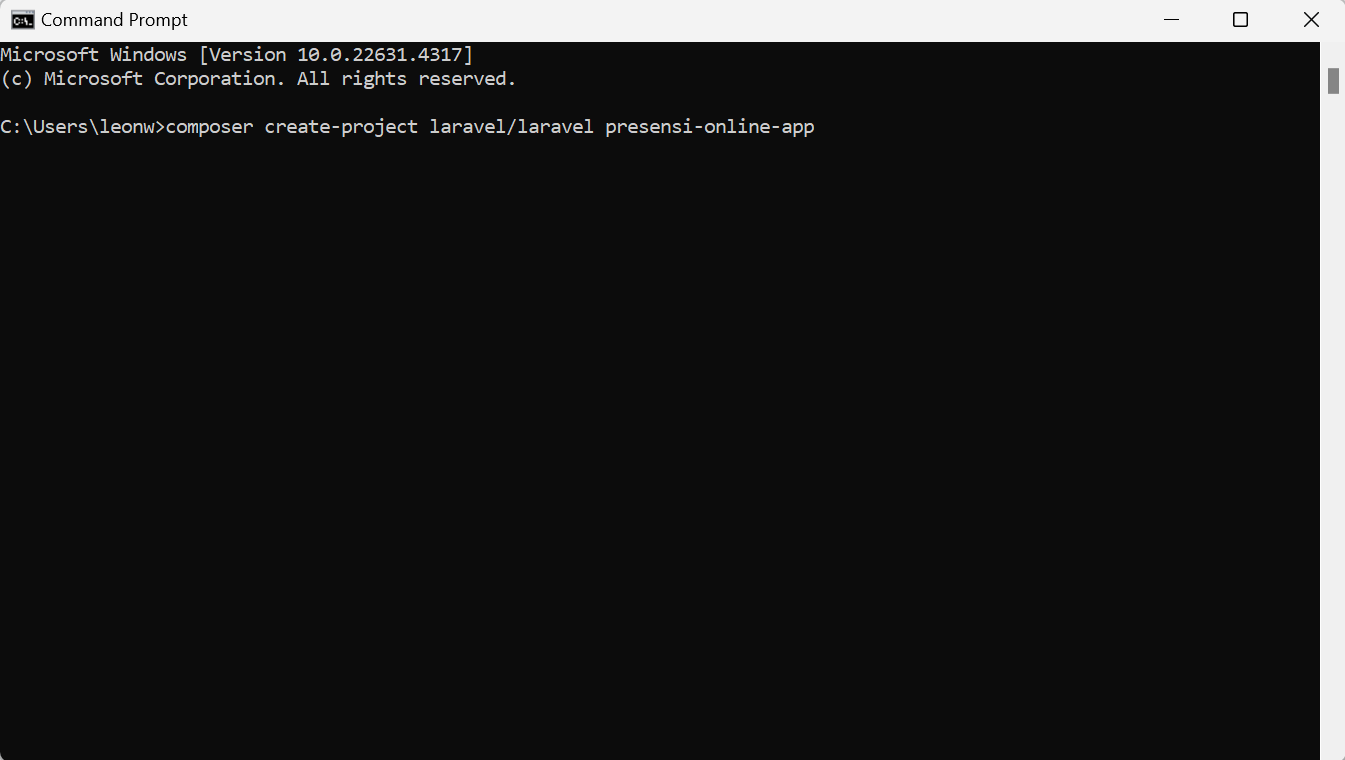
\includegraphics[width=10cm]{Gambar/bab3/command-line-create-laravel.png}
    	\caption{Tampilan \textit{Command Line} Instalasi Laravel}
    	\label{fig:command-line-create-laravel}
    \end{figure}
    \FloatBarrier
    %
Pada pengembangan aplikasi presensi \textit{online} akan menggunakan \textit{Visual Studio Code} sebagai \textit{code editor} yang dapat di-\textit{download} melalui tautan \url{https://code.visualstudio.com/}. \textbf{~\ref{fig:tampilan-laravel-vscode}} menunjukkan tampilan struktur kode Laravel yang dibuka melalui \textit{Visual Studio Code}.
%
    \begin{figure}[!htbp]
    	\centering
    	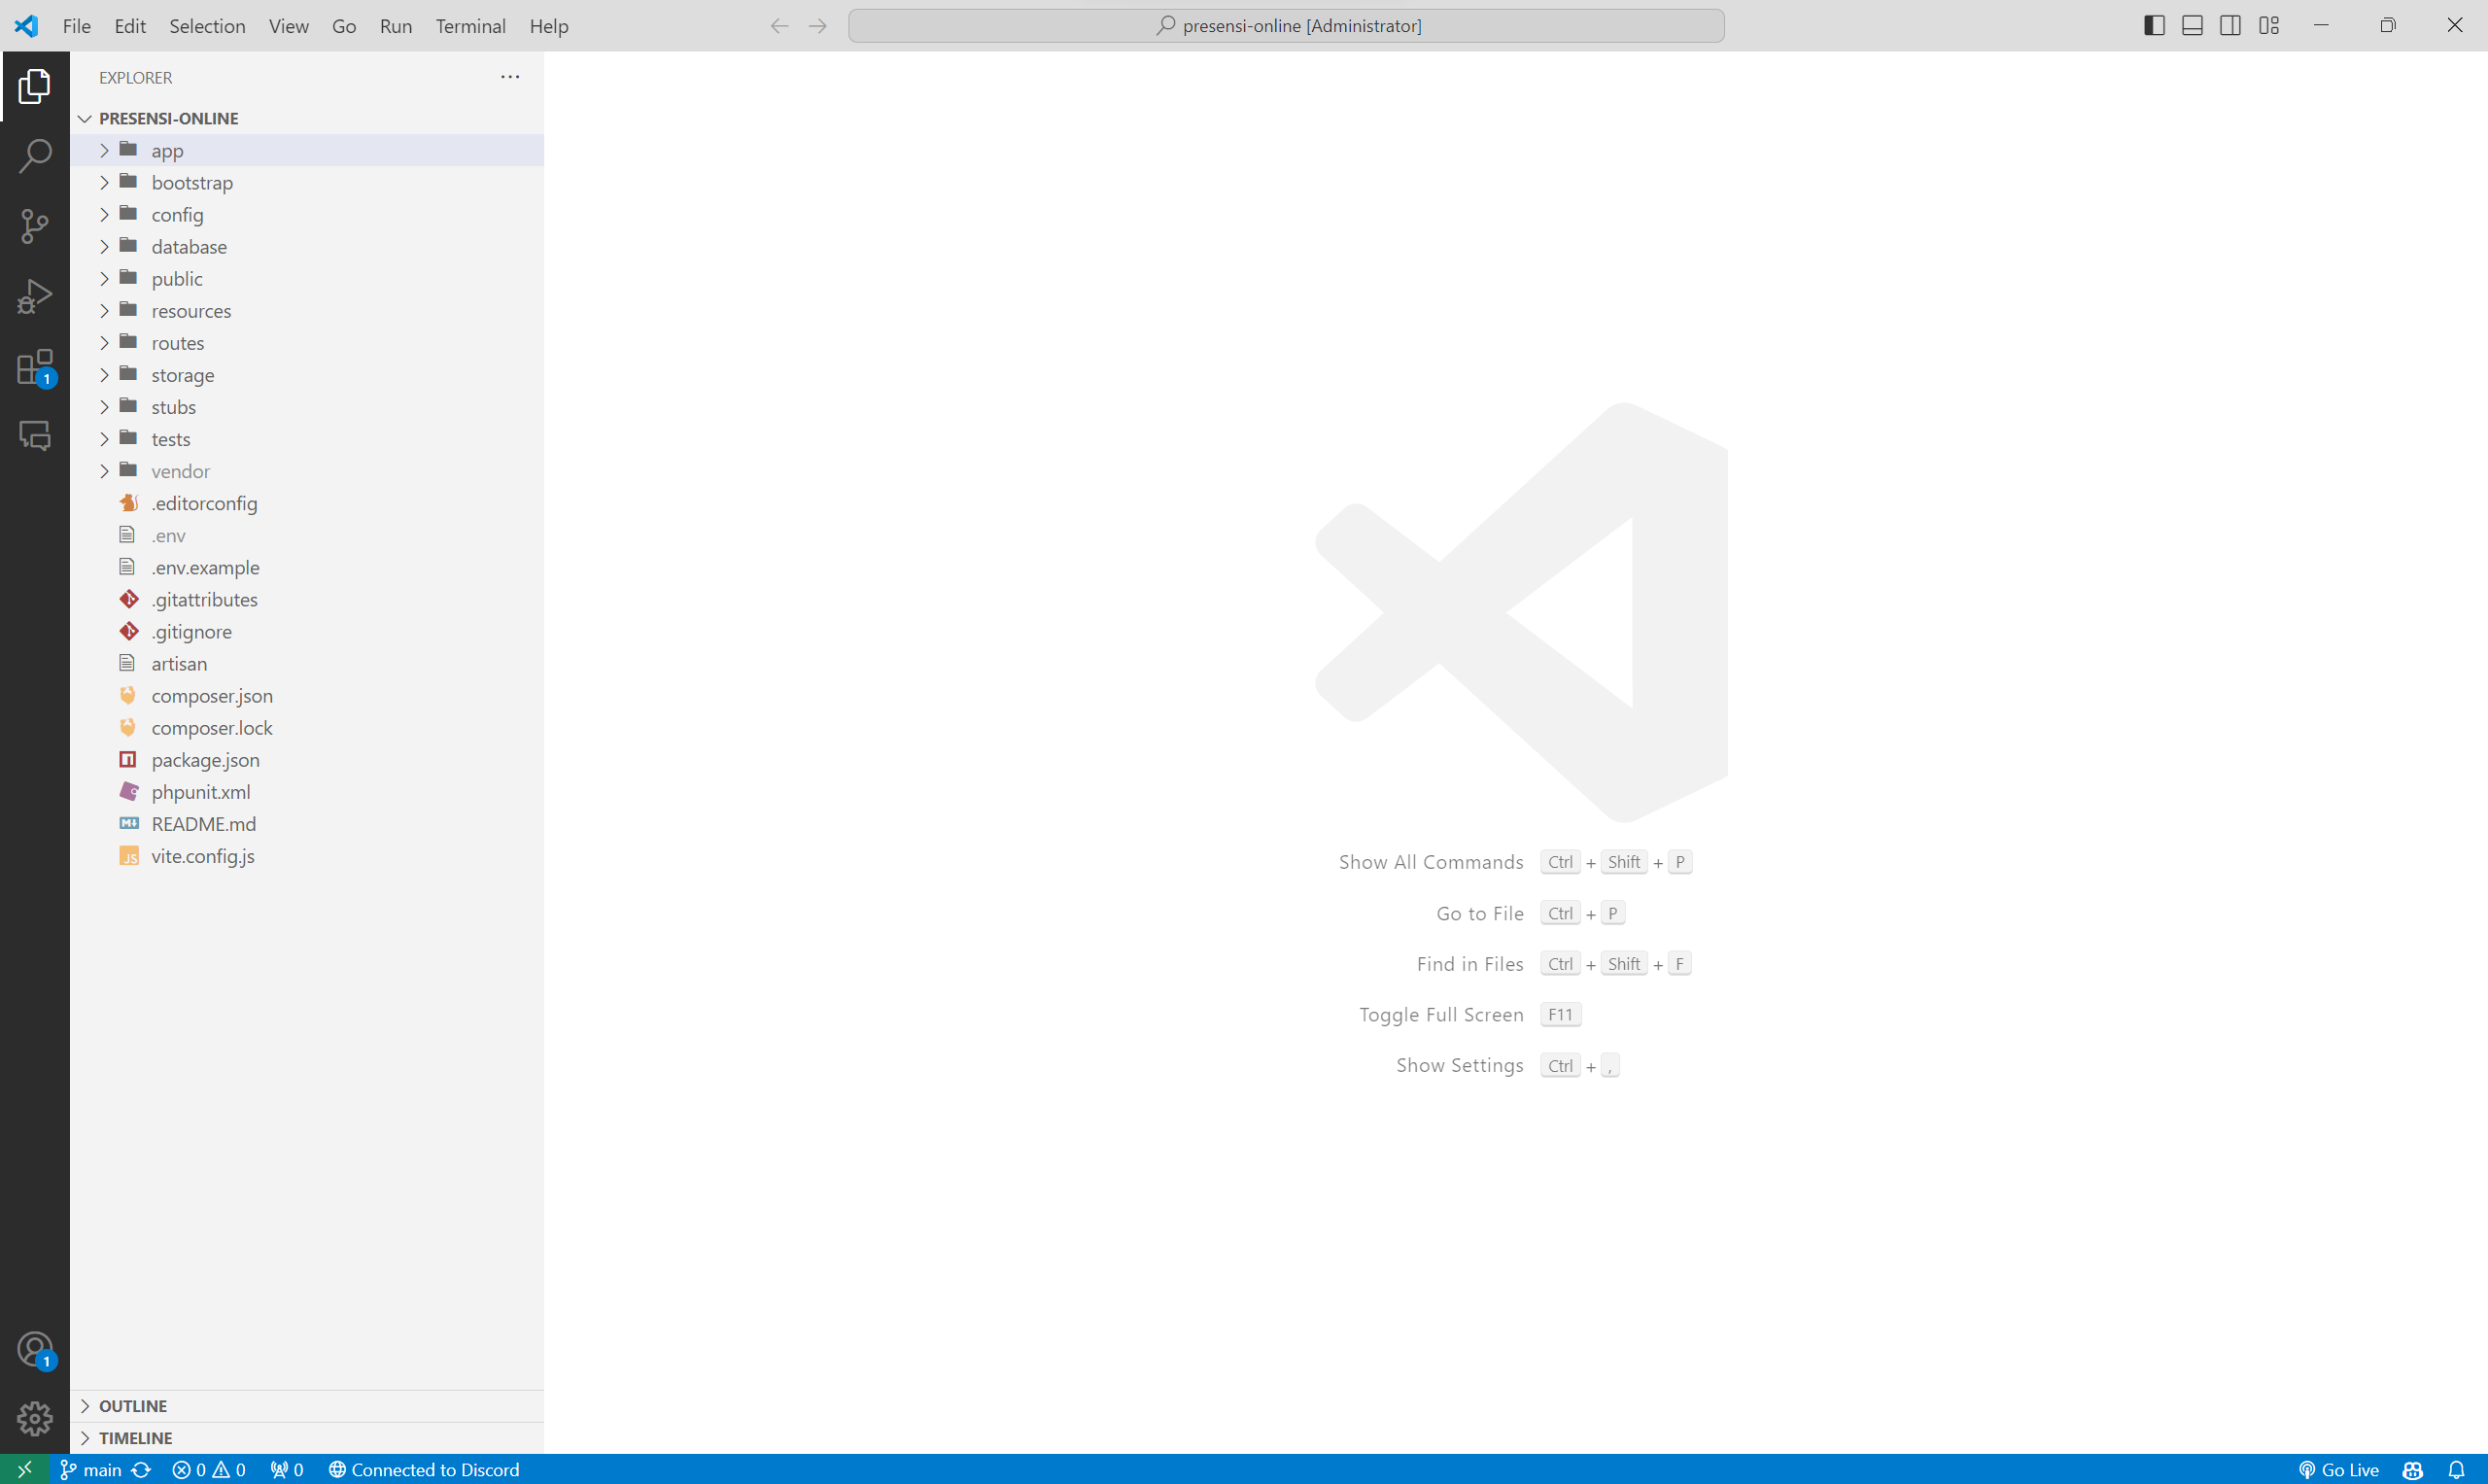
\includegraphics[width=16cm]{Gambar/bab3/code-editor-laravel.png}
    	\caption{Tampilan Struktur Kode Laravel Pada \textit{Visual Studio Code}}
    	\label{fig:tampilan-laravel-vscode}
    \end{figure}
    \FloatBarrier
    %

\subsection{Membuat \textit{Database}}
\textit{Database} yang akan digunakan pada aplikasi ini adalah MySQL. Instalasi MySQL sudah dilakukan bersamaan dengan instalasi XAMPP yang sudah dilakukan pada tahap sebelumnya. Selanjutnya, untuk pembuatan \textit{database} akan menggunakan fitur dari Laravel yaitu \textit{migration}. Sebelumnya, perlu dilakukan konfigurasi \textit{file} .env pada struktur folder Laravel untuk mengatur konfigurasi aplikasi termasuk basis data. \textbf{~\ref{fig:tampilan-file-env}} menampilkan \textit{file} .env yang sudah dikonfigurasi. Laravel menyediakan fitur \textit{migration} untuk membuat tabel pada basis data menggunakan \textit{command line}. \textit{Command line} "php artisan make:model Department -m" merupakan salah satu contoh pembuatan \textit{Model} bersamaan dengan \textit{migration} pada tabel \textit{Department}. Setelah itu mengatur isi kolom yang ingin ditambahkan pada tabel. \textbf{~\ref{fig:tampilan-migration-department}} menunjukkan isi \textit{file migration} yang telah diatur isi kolomnya. Kemudian, jalankan \textit{command line} "php artisan migrate" untuk membuat tabel beserta isi kolomnya. Laravel juga menyediakan fitur \textit{seeder} yang dapat digunakan untuk mengisi baris tabel \textit{Department} dengan menjalankan \textit{command line} "php artisan make:seeder DepartmentSeeder". \textbf{~\ref{fig:tampilan-seeder-department}} menunjukkan isi \textit{file} DepartmentSeeder yang sudah diatur nilainya. Kemudian, jalankan \textit{command line} "php artisan db:seed -class=DepartmentSeeder" untuk memasukkan nilainya ke dalam tabel.
%
    \begin{figure}[!htbp]
    	\centering
    	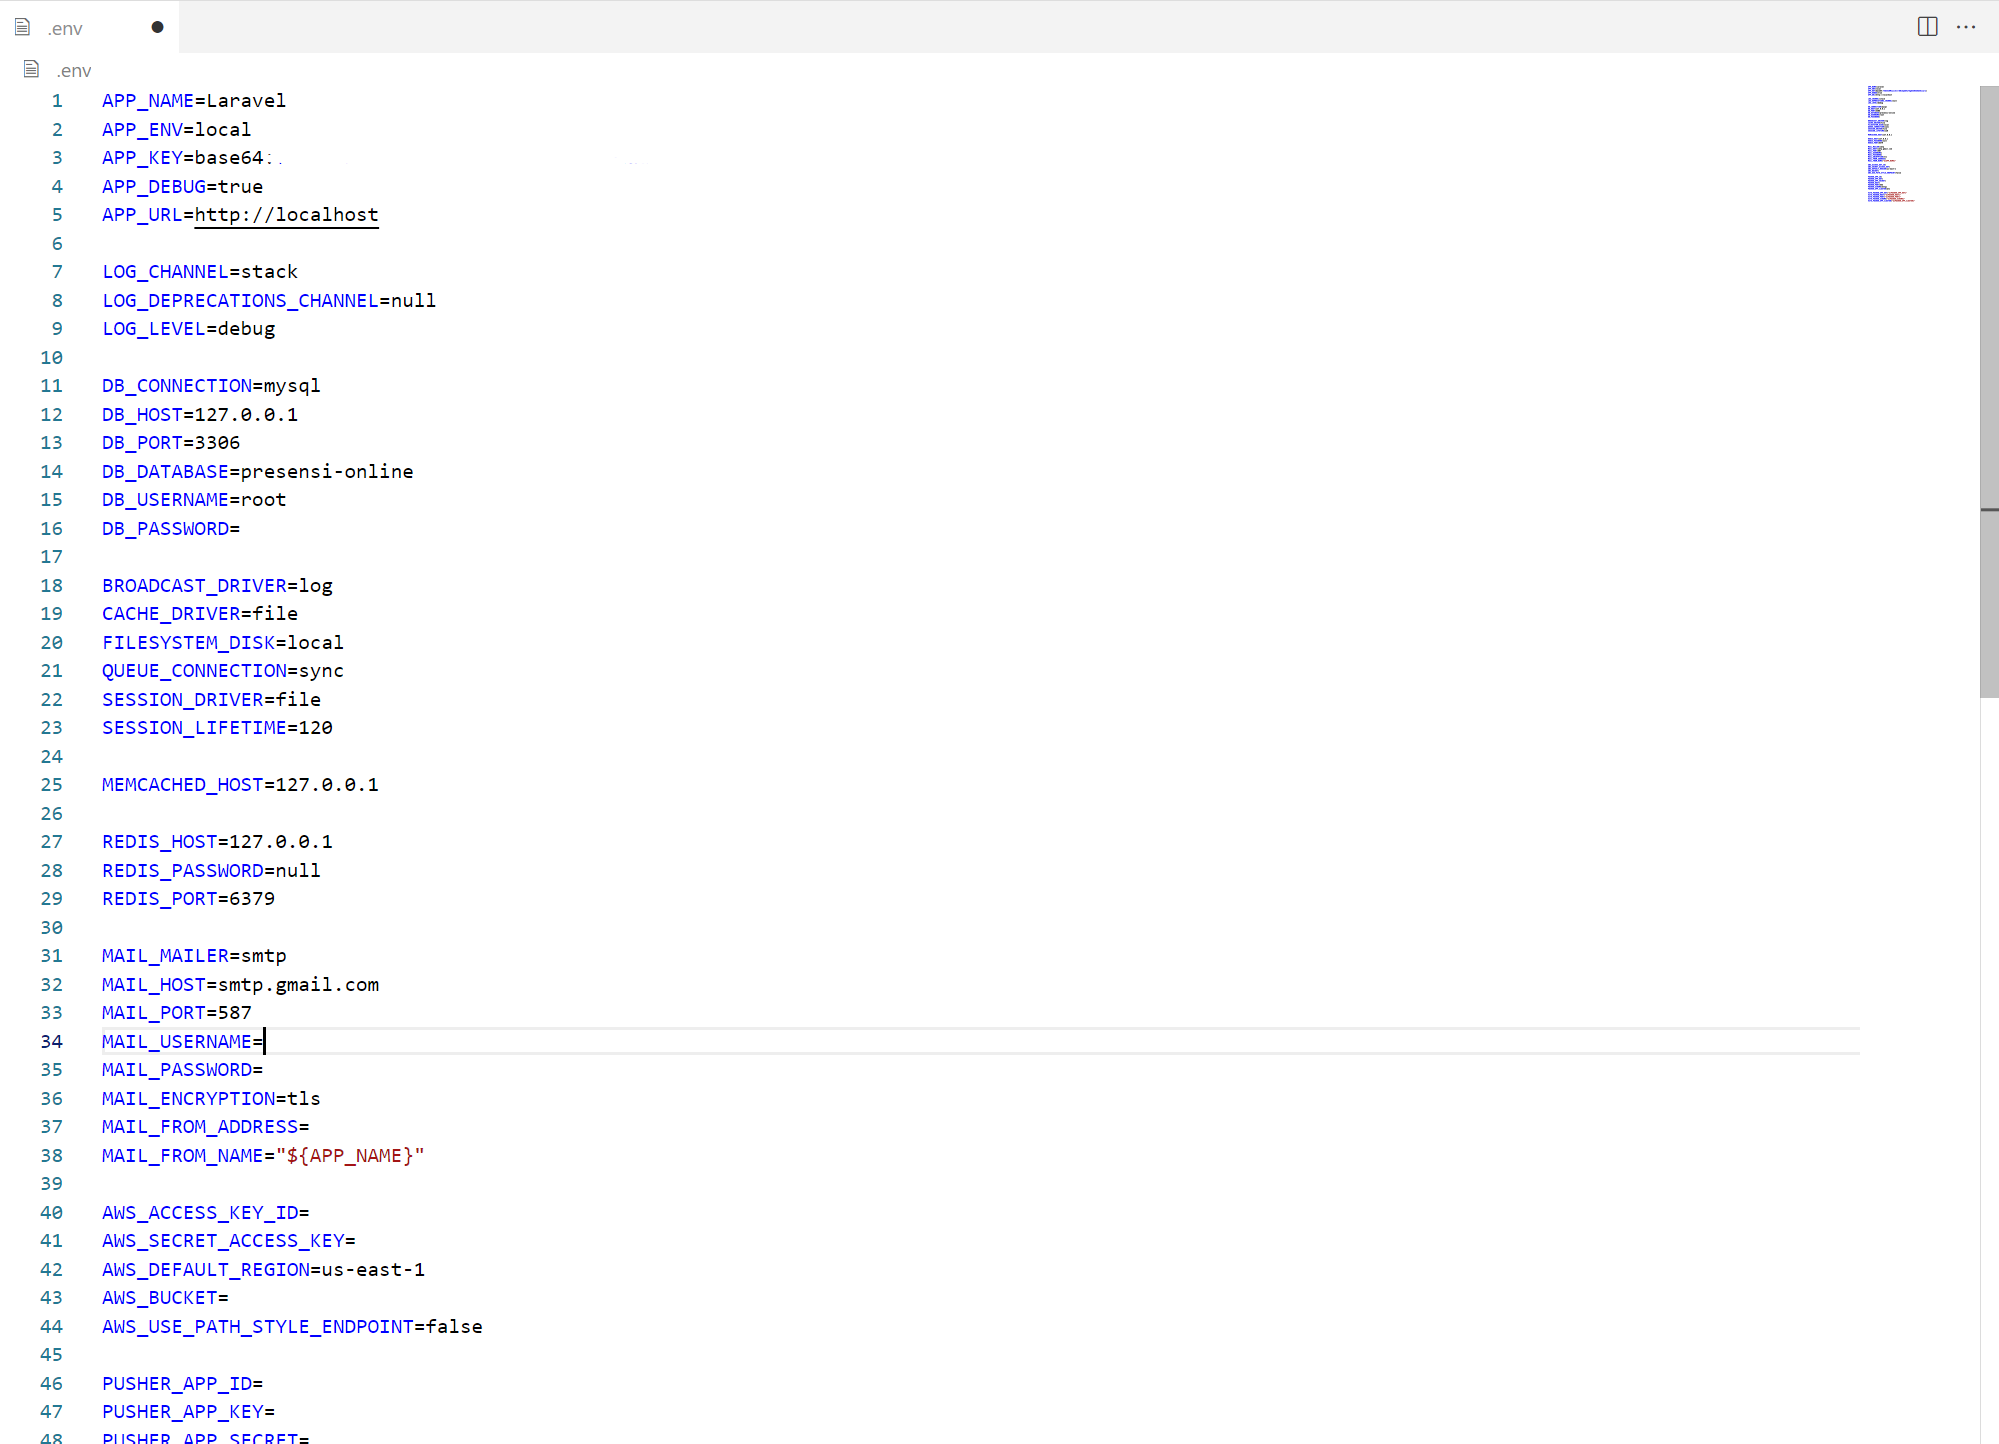
\includegraphics[width=18cm]{Gambar/bab3/file-env.png}
    	\caption{Kode \textit{File} .env}
    	\label{fig:tampilan-file-env}
    \end{figure}
    \FloatBarrier
    %
    %
    \begin{figure}[!htbp]
    	\centering
    	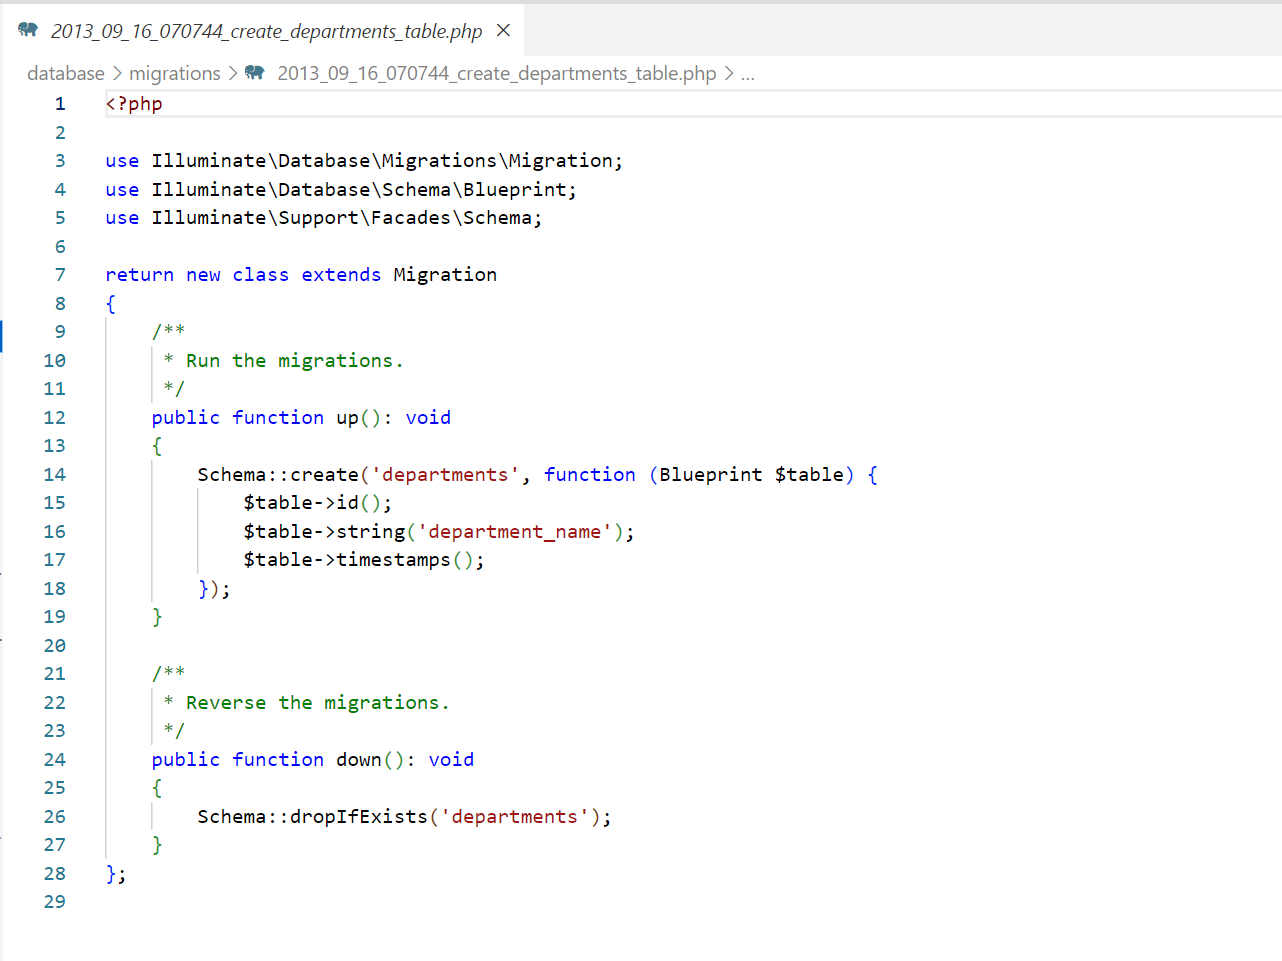
\includegraphics[width=10cm]{Gambar/bab3/migration-department.png}
    	\caption{Kode \textit{Migration} \textit{Department}}
    	\label{fig:tampilan-migration-department}
    \end{figure}
    \FloatBarrier
    %
    %
    \begin{figure}[!htbp]
    	\centering
    	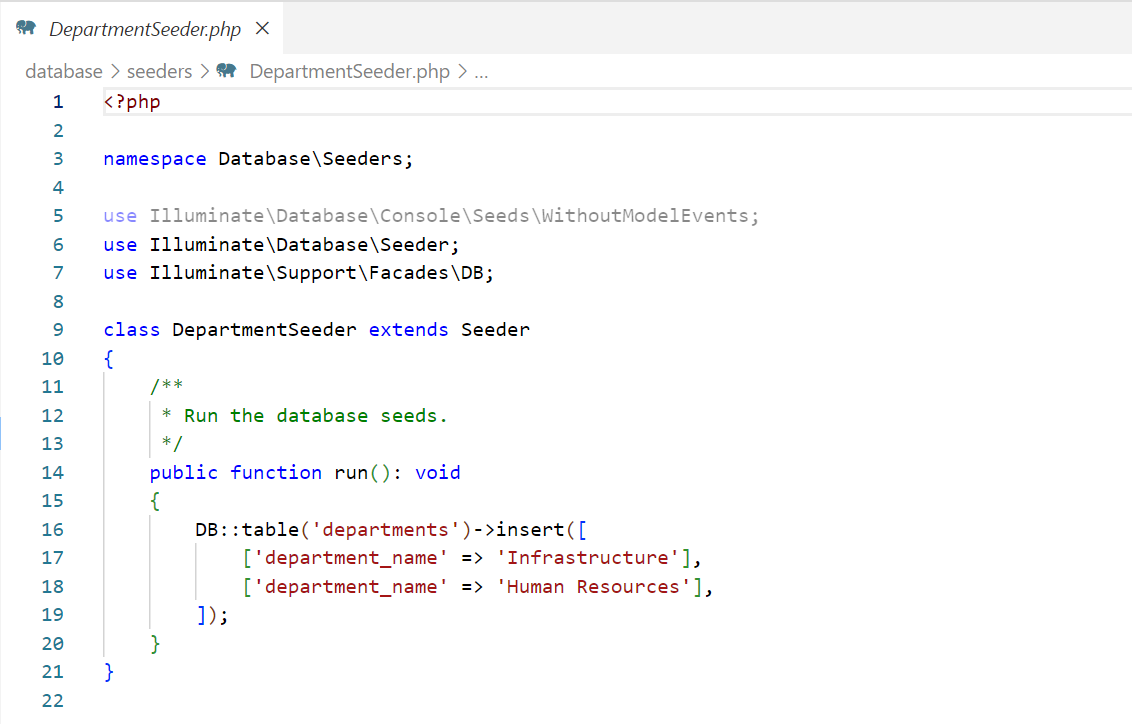
\includegraphics[width=10cm]{Gambar/bab3/seeder-department.png}
    	\caption{Kode \textit{Seeder} \textit{Department}}
    	\label{fig:tampilan-seeder-department}
    \end{figure}
    \FloatBarrier
    %

\subsection{Implementasi Setiap Modul Pada Aplikasi}
Pengembangan aplikasi presensi \textit{online} akan dilakukan per modul seperti modul presensi, \textit{shift}, riwayat presensi, riwayat lembur, dan modul lainnya. Pengembangan aplikasi akan menggunakan \textit{framework} Laravel yang menerapkan konsep MVC (\textit{Model-View-Controller}). \textit{Model} merupakan komponen yang berfungsi mengelola data dan logika bisnis aplikasi. \textit{Model} berinteraksi dengan \textit{database} untuk menyimpan, mengambil, dan memproses data. Dalam Laravel, terdapat \textit{Eloquent} ORM, yang memungkinkan manipulasi data tanpa menulis SQL secara langsung. \textit{View} merupakan bagian yang bertanggung jawab untuk menampilkan data kepada pengguna dalam bentuk antarmuka pengguna (UI) menggunakan Laravel \textit{Templating Engine}. \textit{Styling} dari setiap modul akan menggunakan \textit{framework} Tailwind CSS dan \textit{library Flowbite}, selain itu, tampilan \textit{pop up} pesan akan menggunakan \textit{library Sweet Alert}. \textit{Controller} berperan sebagai penghubung antara \textit{model} dan \textit{view}. \textit{Controller} menerima \textit{input} dari pengguna (biasanya melalui \textit{request} HTTP), memprosesnya dengan bantuan \textit{model}, dan mengembalikan data ke \textit{view} untuk ditampilkan. Selain itu, terdapat juga \textit{routes} yang akan merespons permintaan HTTP dan menjadi penghubung permintaan tersebut dengan \textit{controller}.

Implementasi setiap modul akan dimulai dengan membuat \textit{controller} yang merupakan \textit{backend} pada aplikasi. Salah satu contoh pembuatan \textit{controller} untuk modul \textit{department} dilakukan dengan menjalankan \textit{command line} "php artisan make:controller DepartmentController". \textbf{~\ref{fig:tampilan-controller-department}} menunjukkan isi \textit{file controller} yang akan mengembalikan ke \textit{view department}. Selanjutnya, daftarkan masing-masing \textit{function} dalam \textit{controller} ke \textit{routes} agar dapat diakses melalui permintaan HTTP. \textbf{~\ref{fig:tampilan-routes-department}} menampilkan kode \textit{routes} agar \textit{controller} pada \textit{function index} dapat diakses melalui permintaan HTTP. Selanjutnya membuat tampilan UI atau \textit{view} menggunakan \textit{blade templating engine} dengan cara membuat \textit{file} baru bernama department.blade.php pada \textit{folder view} kemudian didalamnya berisi kode HTML yang nantinya akan ditampilkan jika pengguna mengakses \textit{route} yang telah ditentukan. \textbf{~\ref{fig:kode-view-department}} menunjukkan kode HTML pada \textit{file department.blade.php} yang dibuat menggunakan \textit{blade templating engine}. \textbf{~\ref{fig:tampilan-view-department}} merupakan tampilan halaman \textit{Department} yang diakses melalui \textit{routes} sebelumnya. 
%
    \begin{figure}[!htbp]
    	\centering
    	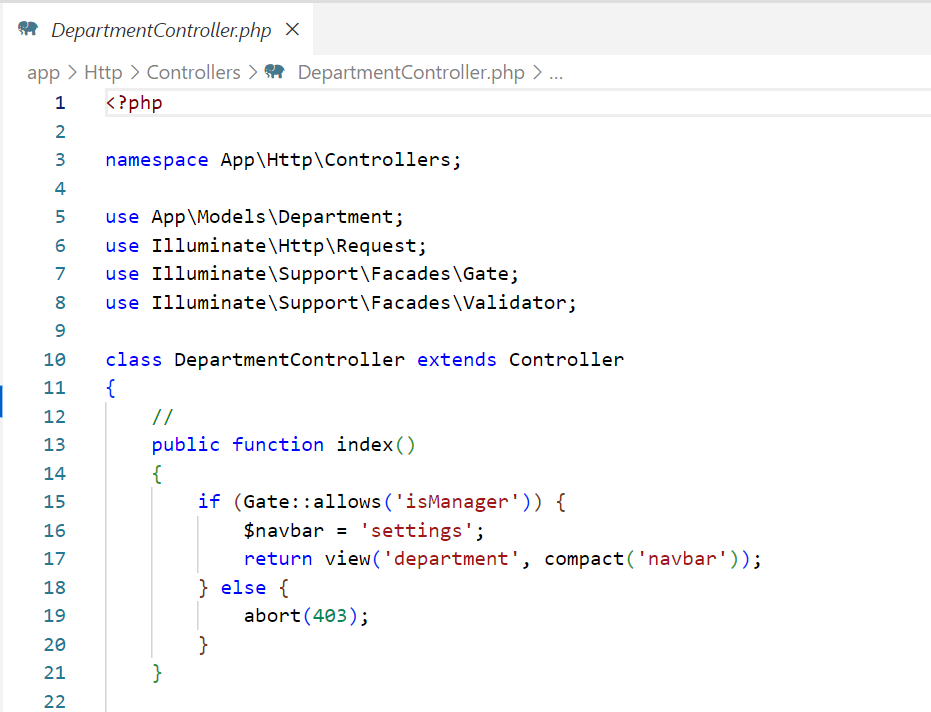
\includegraphics[width=10cm]{Gambar/bab3/controller-department.png}
    	\caption{Kode \textit{Controller} \textit{Department}}
    	\label{fig:tampilan-controller-department}
    \end{figure}
    \FloatBarrier
%
%
    \begin{figure}[!htbp]
    	\centering
    	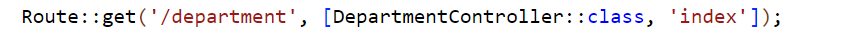
\includegraphics[width=10cm]{Gambar/bab3/routes-department.png}
    	\caption{Kode \textit{Routes} \textit{Department}}
    	\label{fig:tampilan-routes-department}
    \end{figure}
    \FloatBarrier
%
%
    \begin{figure}[!htbp]
    	\centering
    	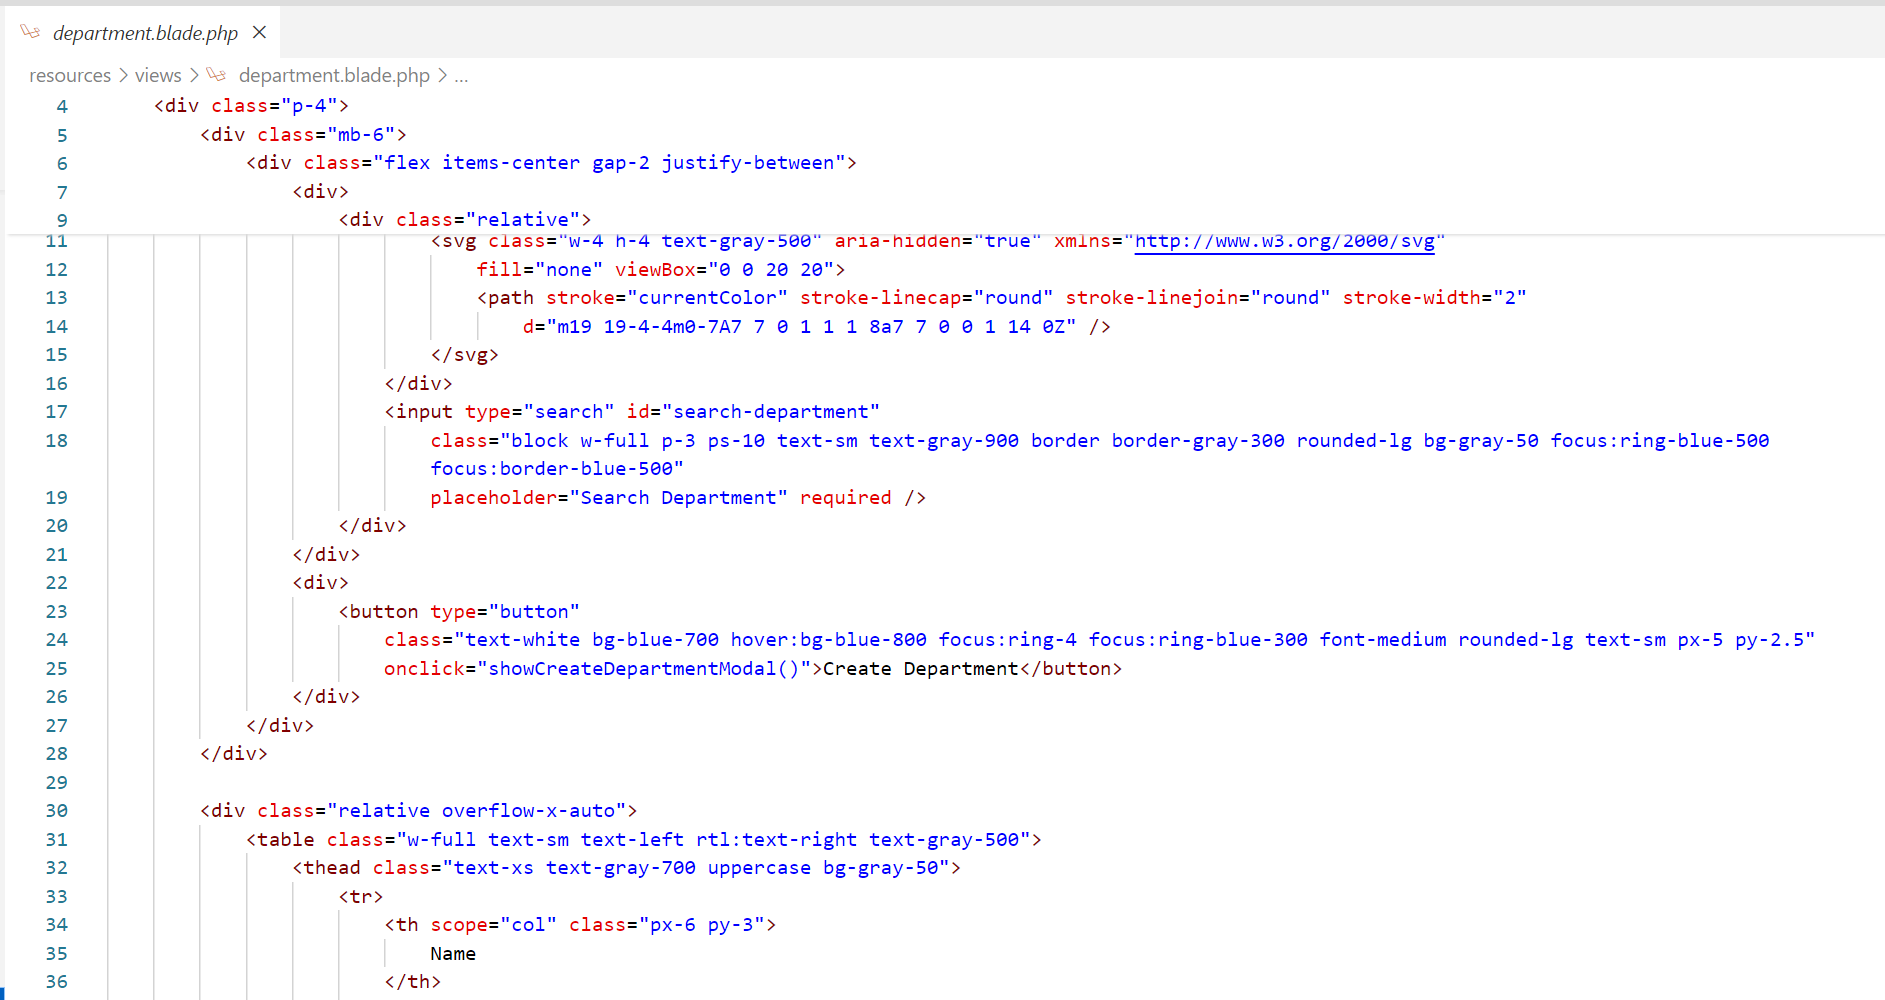
\includegraphics[width=10cm]{Gambar/bab3/view-department.png}
    	\caption{Kode \textit{View} \textit{Department}}
    	\label{fig:kode-view-department}
    \end{figure}
    \FloatBarrier
%
%
    \begin{figure}[!htbp]
    	\centering
    	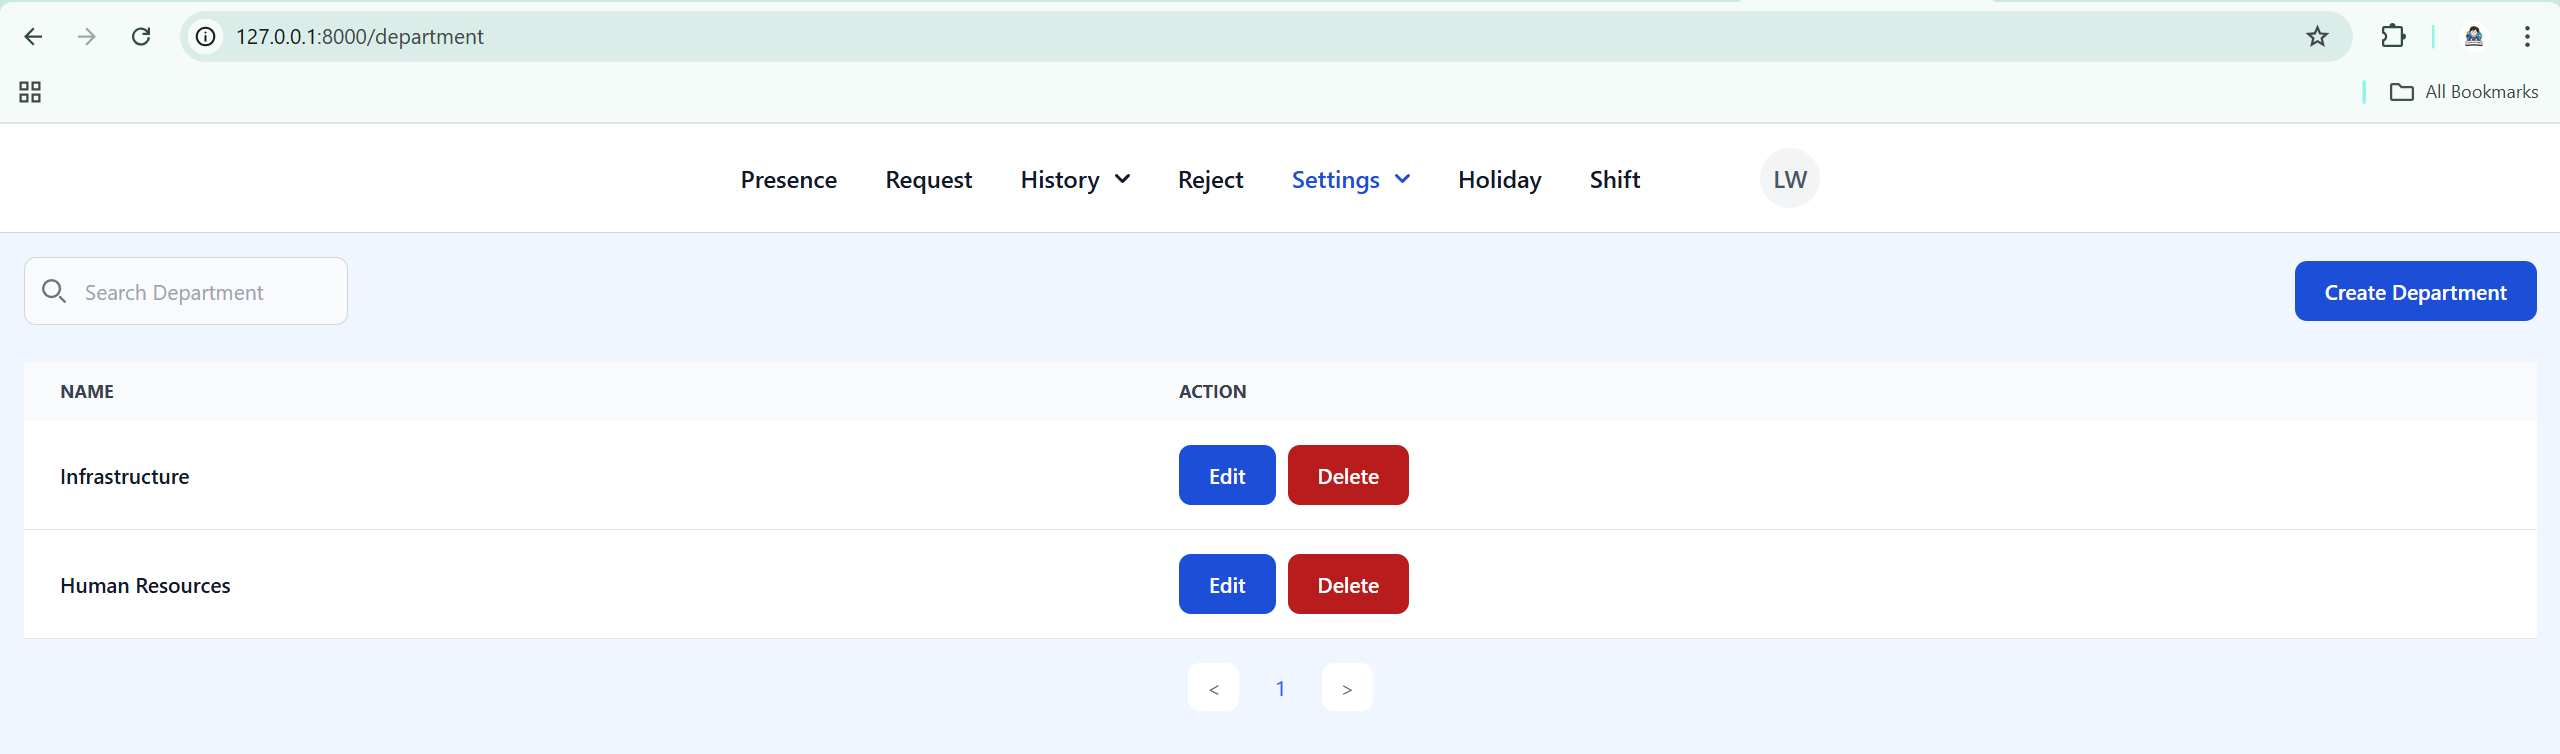
\includegraphics[width=12cm]{Gambar/bab3/tampilan-view-department.png}
    	\caption{Tampilan Halaman \textit{Department}}
    	\label{fig:tampilan-view-department}
    \end{figure}
    \FloatBarrier
%

%
    \begin{figure}[!htbp]
    	\centering
    	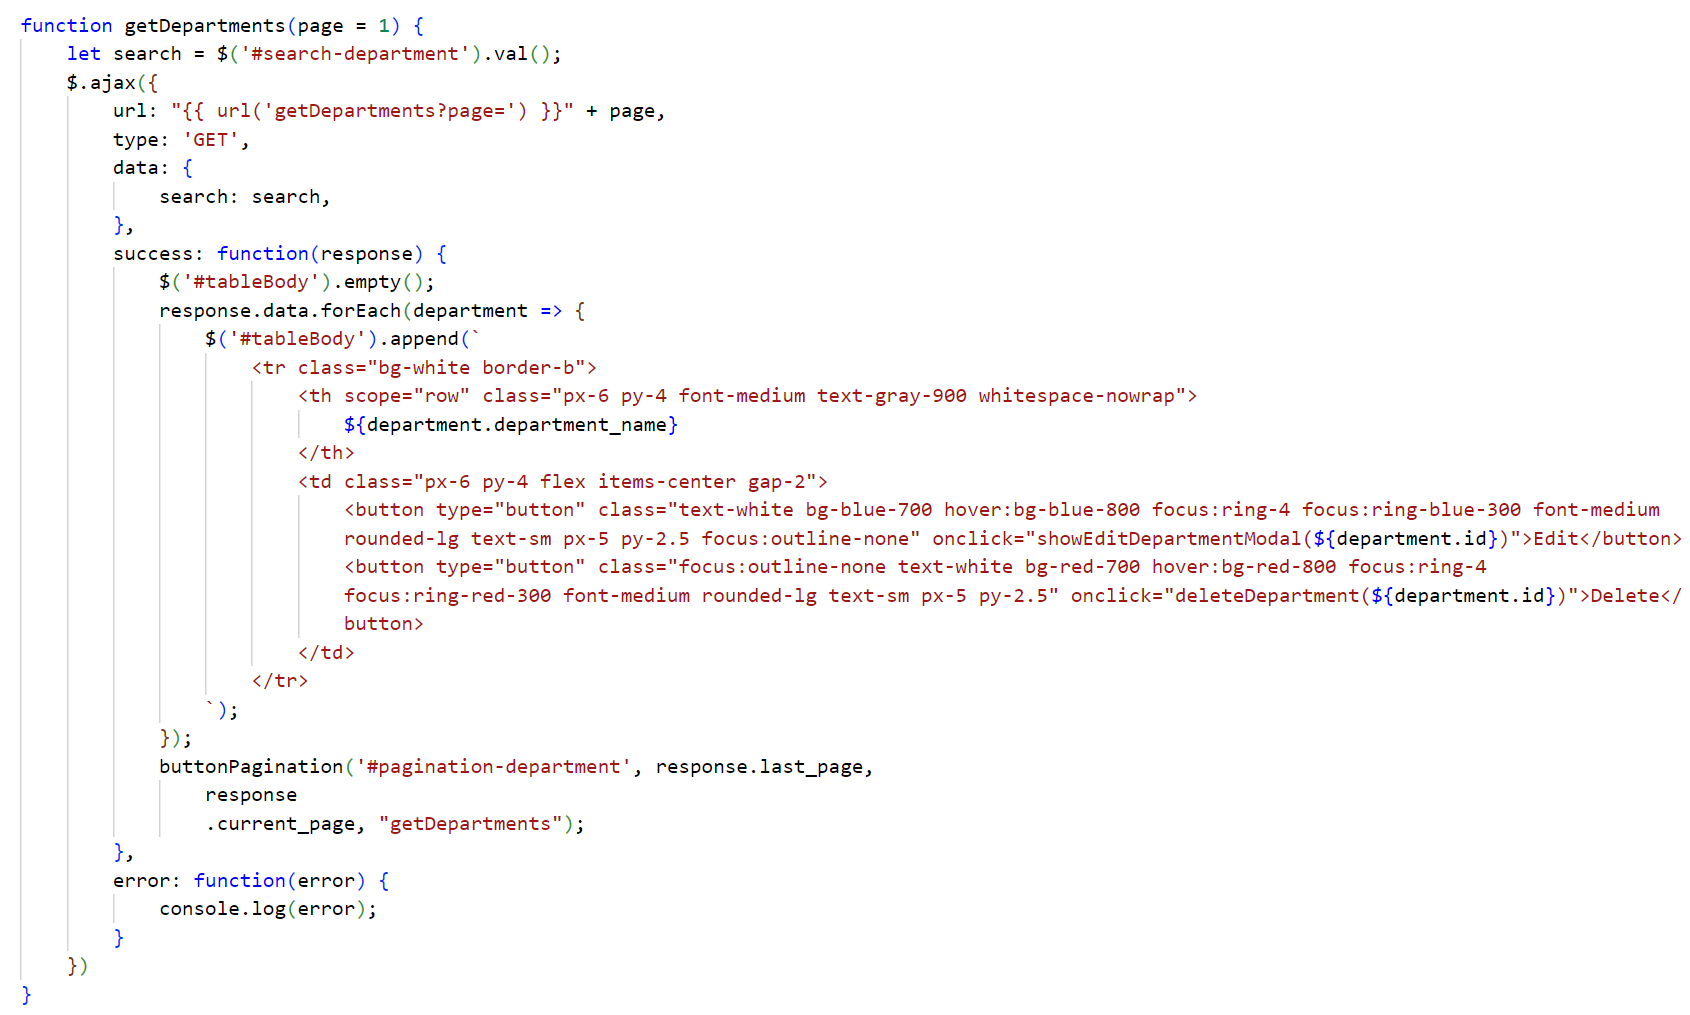
\includegraphics[width=12cm]{Gambar/bab3/ajax-department.png}
    	\caption{Kode AJAX \textit{Fetch} Data \textit{Department}}
    	\label{fig:kode-ajax-department}
    \end{figure}
    \FloatBarrier
%
Dalam setiap modul, pengambilan data akan dilakukan secara terpisah dengan \textit{controller} yang mengembalikan \textit{view}. Pengambilan data akan menggunakan bantuan \textit{library} JavaScript yaitu Jquery AJAX untuk melakukan permintaan HTTP secara \textit{asynchronus} sehingga ketika terjadi penambahan, pengubahan, dan penghapusan data maka halaman tidak ada dimuat kembali melainkan data akan otomatis ter-\textit{update} pada sisi server. \textbf{~\ref{fig:kode-ajax-department}} menampilkan \textit{function} untuk mengambil data \textit{department} secara \textit{asynchronus} menggunakan JQuery AJAX.

\subsection{Implementasi \textit{Geolocation}}
Aplikasi presensi \textit{online} akan mengimplementasi teknologi \textit{Geolocation} untuk mendapatkan titik koordinat lokasi pengguna. Dalam HTML terdapat \textit{Geolocation} API yang dapat digunakan melalui JavaScript tanpa harus meng-\textit{install plugin} tambahan. Dokumenasi penggunaan \textit{Geolocation} API dapat dilihat melalui tautan \url{https://www.w3schools.com/html/html5_geolocation.asp}. \textit{Geolocation} API telah mendukung sebagian banyak \textit{browser modern} seperti \textit{Google Chrome, Safari,} dan lain-lain. \textbf{\ref{fig:kode-geolocation-api}} menunjukkan contoh penggunaan \textit{Geolocation} API pada aplikasi presensi \textit{online} untuk mendapatkan titik koordinat lokasi pengguna.
 \begin{figure}[!htbp]
    	\centering
    	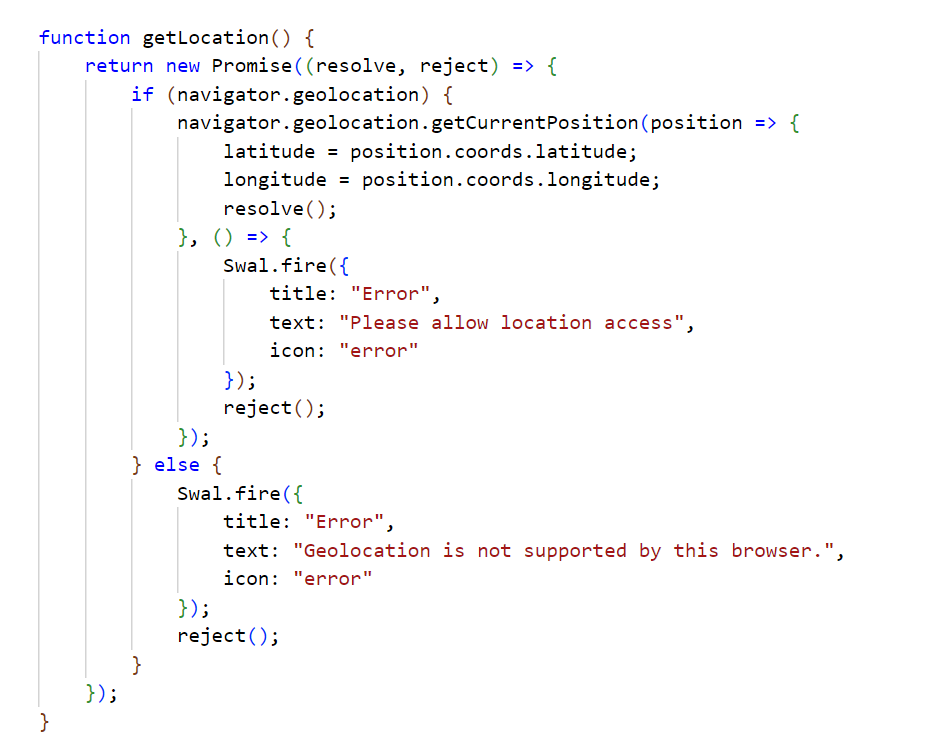
\includegraphics[width=10cm]{Gambar/bab3/kode-geolocation.png}
    	\caption{Kode \textit{Geolocation} API}
    	\label{fig:kode-geolocation-api}
    \end{figure}
    \FloatBarrier

\subsection{Implementasi Peta Interaktif}
Pada aplikasi presensi \textit{online} terdapat gambar peta yang ditampilkan kepada \textit{Staff Infrastructure} saat melakukan presensi. Fungsi peta ini agar \textit{Staff Infrastructure} dapat mengetahui apakah lokasi sudah sesuai dengan posisinya. \textit{library }Leaflet JS akan digunakan pada aplikasi presensi \textit{online} untuk menampilkan gambar peta lokasi \textit{staff}. Dokumentasi \textit{library} Leaflet JS dapat dilihat melalui tautan \url{https://leafletjs.com/reference.html}. Penggunaan \textit{library} Leaflet JS hanya perlu membutuhkan parameter titik koordinat lokasi \textit{Staff Infrastructure} berupa \textit{longitude} dan \textit{latitude} yang telah didapatkan melalui teknologi \textit{Geolocation} API sebelumnya. \textbf{\ref{fig:hasil-leaflet-js}} menunjukkan gambar titik lokasi pengguna yang ditampilkan dalam bentuk peta menggunakan \textit{library} Leaflet JS.
\begin{figure}[!htbp]
    	\centering
    	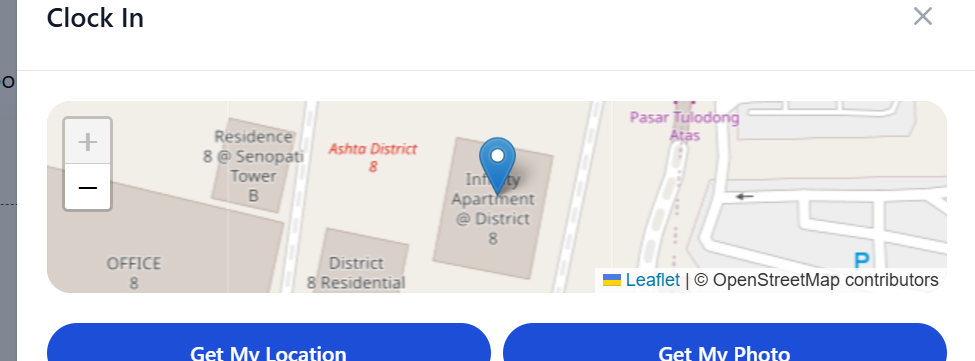
\includegraphics[width=15cm]{Gambar/bab3/hasil-leaflet-js.png}
    	\caption{Hasil Gambar Peta Lokasi Menggunakan Leaflet JS}
    	\label{fig:hasil-leaflet-js}
    \end{figure}
    \FloatBarrier
    
\subsection{Implementasi Perhitungan Jarak}
Aplikasi ini akan mengimplementasikan algoritma Haversine. Algoritma Haversine akan digunakan untuk menghitung jarak antara lokasi pengguna saat presensi dengan lokasi kantor. Lokasi pengguna akan didapatkan melalui teknologi \textit{Geolocation} API yang telah diimplementasikan sebelumnya. Hasil dari perhitungan akan memberikan keterangan pada presensi yaitu "\textit{In Office}" jika pengguna melakukan presensi di sekitar radius kantor dan "\textit{Out Office}" jika pengguna melakukan presensi di luar radius kantor. Jarak toleransi akan diberikan sebesar 120 meter. \textbf{~\ref{fig:kode-function-haversine}} menunjukkan kode \textit{function} Haversine yang akan digunakan untuk menghitung kedua jarak. \textbf{~\ref{fig:tampilan-keterangan-presensi}} menampilkan tampilan keterangan presensi yaitu "\textit{In Office}" dan "\textit{Out Office}" yang didapat melalui perhitungan algoritma Haversine pada halaman riwayat presensi.
%
    \begin{figure}[!htbp]
    	\centering
    	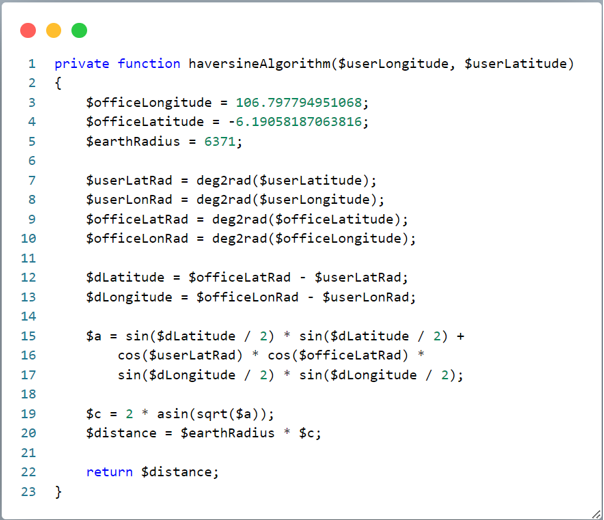
\includegraphics[width=10cm]{Gambar/bab3/function-haversine.png}
    	\caption{Kode \textit{Function} Haversine}
    	\label{fig:kode-function-haversine}
    \end{figure}
    \FloatBarrier
%
%
    \begin{figure}[!htbp]
    	\centering
    	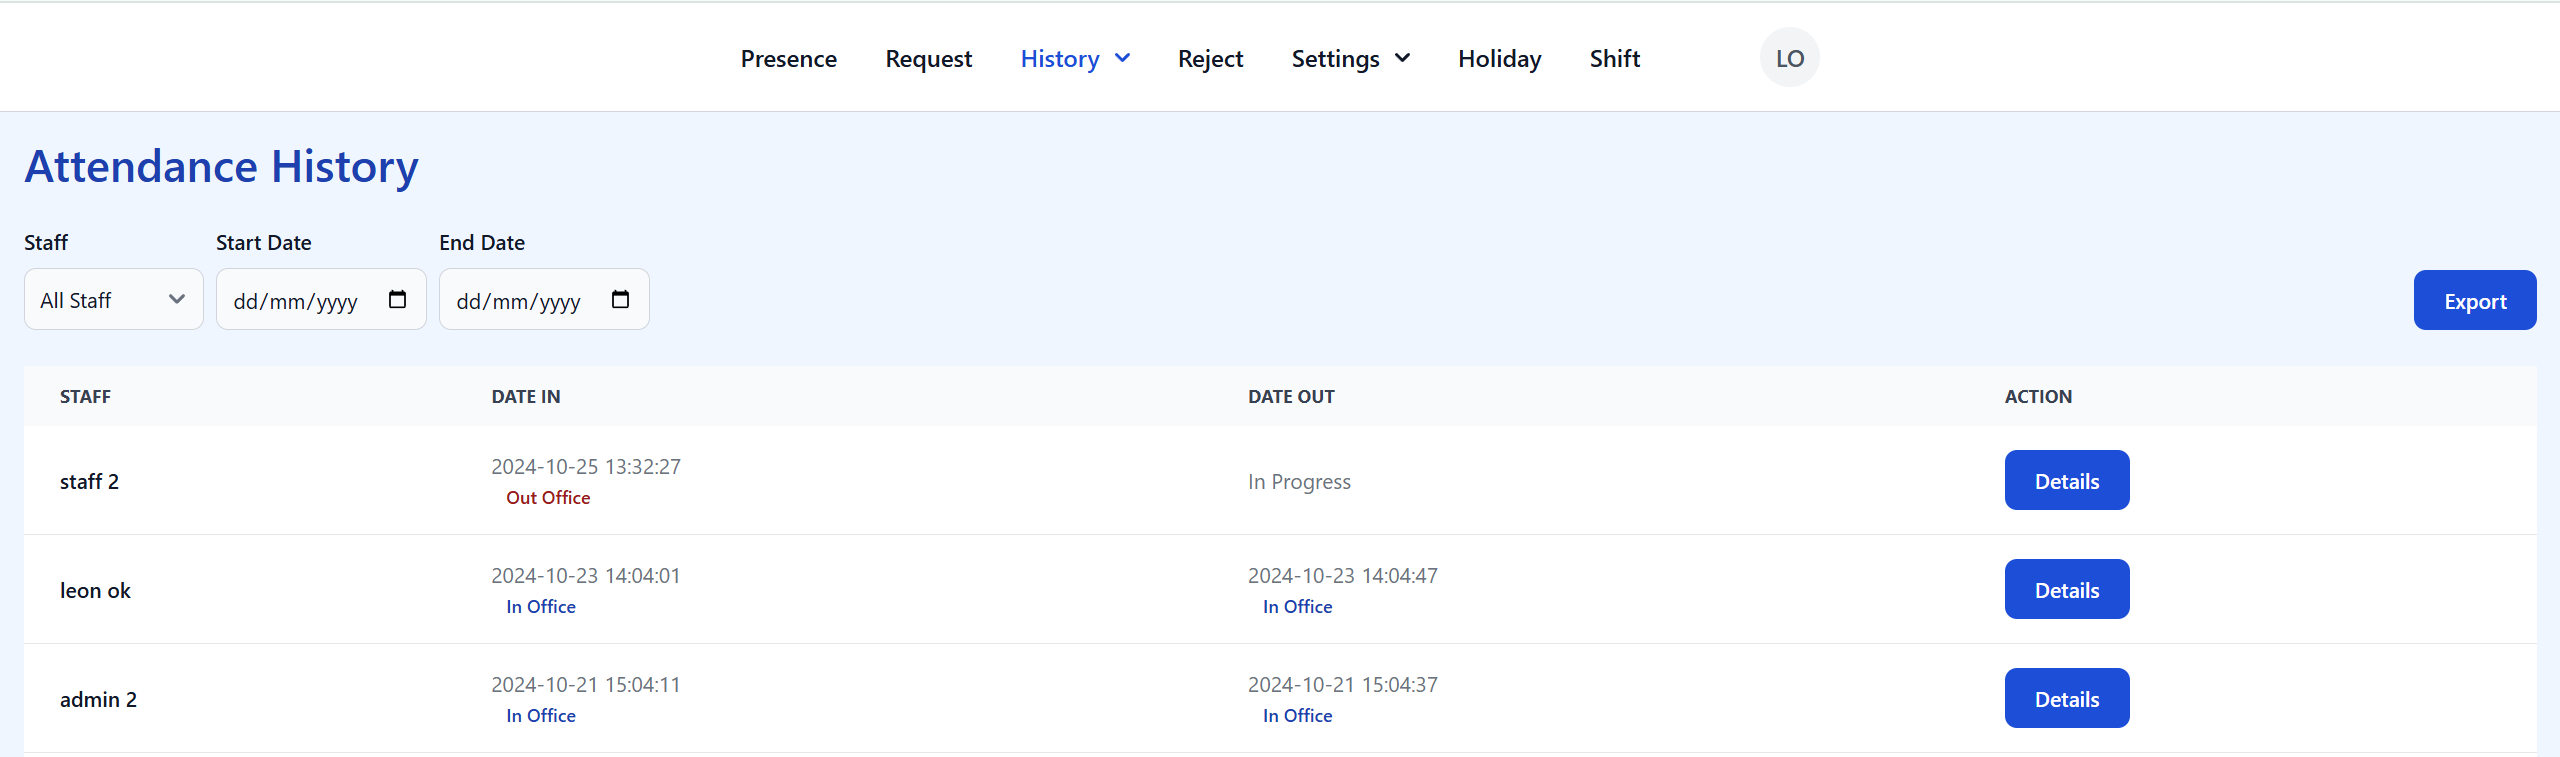
\includegraphics[width=15cm]{Gambar/bab3/tampilan-keterangan-presensi.png}
    	\caption{Tampilan Keterangan Presensi}
    	\label{fig:tampilan-keterangan-presensi}
    \end{figure}
    \FloatBarrier
%



\subsection{Implementasi Validasi Wajah}
Pada aplikasi presensi \textit{online} akan terdapat fitur untuk pengambilan wajah saat \textit{staff} melakukan presensi. Aplikasi presensi akan menggunakan teknologi WebRTC sebagai kamera menggunakan JavaScript tanpa perlu meng-\textit{install} \textit{plugin} tambahan. Penggunaan teknologi WebRTC ini agar pengambilan wajah dilakukan secara langsung saat presensi sehingga tidak terjadi kecurangan seperti meng-\textit{upload file} foto pada galeri pengguna. \textbf{\ref{fig:kode-webrtc}} menunjukkan kode \textit{function} untuk membuka mengakses kamera depan menggunakan teknologi WebRTC.
\begin{figure}[!htbp]
    	\centering
    	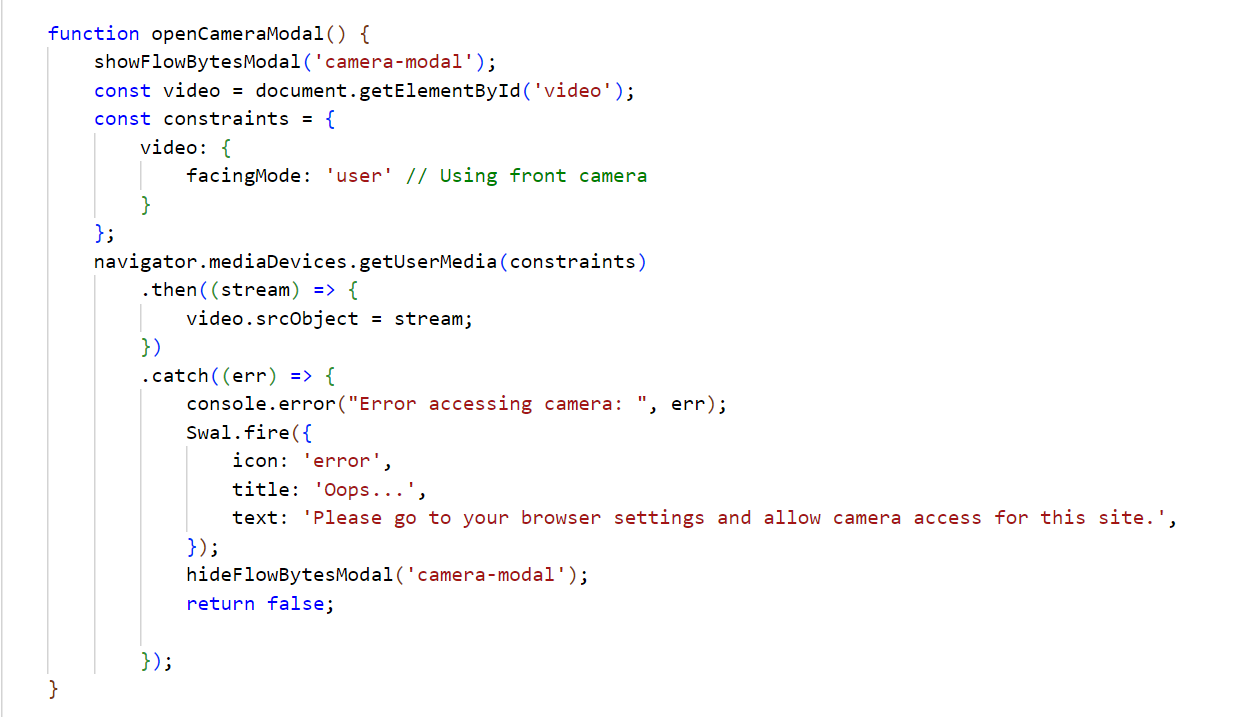
\includegraphics[width=15cm]{Gambar/bab3/kode-webrtc-kamera.png}
    	\caption{Kode WebRTC Pada Kamera}
    	\label{fig:kode-webrtc}
    \end{figure}
    \FloatBarrier
Selain itu, aplikasi presensi \textit{online} akan menerapkan TensorFlow. TensorFlow merupakan \textit{framework open-source} yang dikembangkan oleh \textit{Google} untuk komputasi numerik dan \textit{machine learning}, terutama \textit{deep learning}. Pada aplikasi presensi \textit{online} akan menerapkan \textit{model BlazeFace} yang merupakan \textit{model deep learning} yang dikembangkan oleh \textit{Google} untuk mendeteksi wajah dengan cepat dan efisien, terutama pada perangkat seluler. Penggunaan \textit{model} ini cukup mudah yaitu dengan menyisipkan kode script CDN pada aplikasi yang dapat dilihat pada \textbf{~\ref{fig:kode-script-cdn-tensorflow}}.
%
    \begin{figure}[!htbp]
    	\centering
    	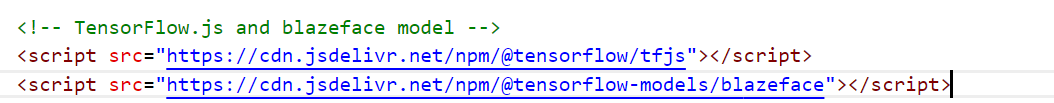
\includegraphics[width=15cm]{Gambar/bab3/cdn-tensorflow.png}
    	\caption{Kode Script CDN TensorFlow dan \textit{Model BlazeFace}}
    	\label{fig:kode-script-cdn-tensorflow}
    \end{figure}
    \FloatBarrier
%
Setelah itu, memasukkan kode logika yang digunakan untuk mengecek wajah pada saat pengambilan foto melalui kamera saat presensi. \textbf{~\ref{fig:kode-function-pengambilan-foto}} menunjukkan kode pengambilan foto saat presensi, dalam \textit{function} tersebut akan dilakukan pengecekkan wajah pada kamera menggunakan TensorFlow. Foto yang diambil akan divalidasi seperti harus terdapat wajah pada kamera, tidak boleh terlalu dekat dengan kamera, dan posisi wajah harus berada ditengah kamera saat pengambilan foto.
%
    \begin{figure}[!htbp]
    	\centering
    	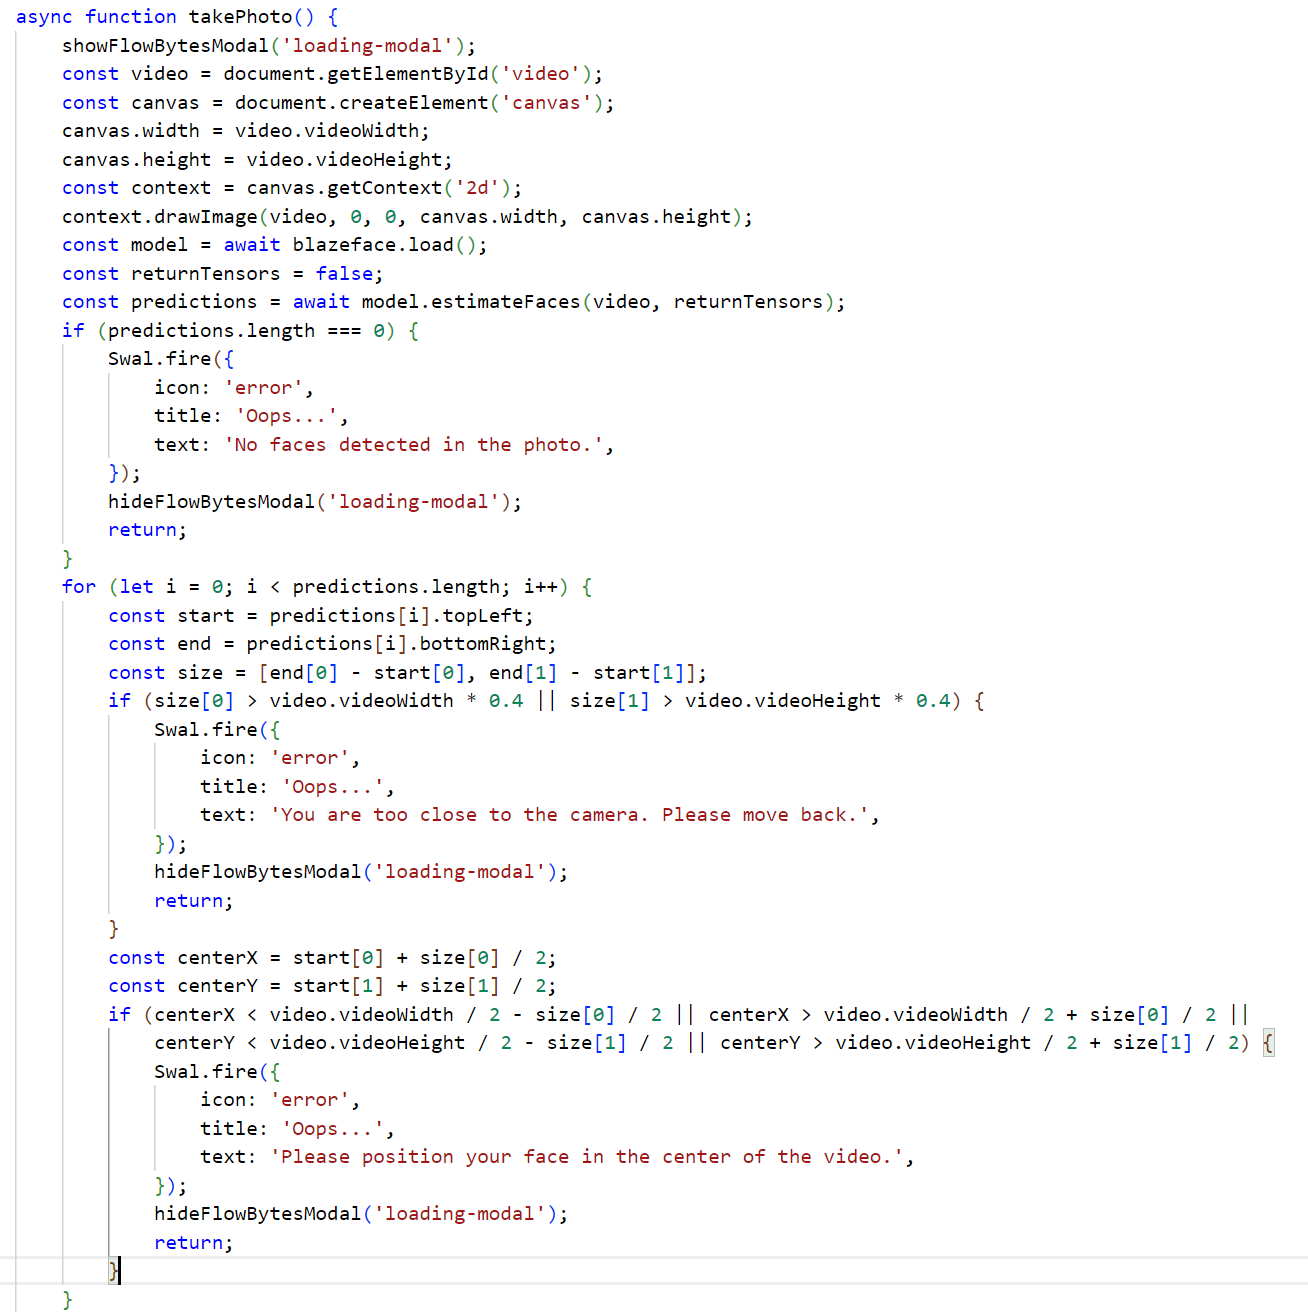
\includegraphics[width=9cm]{Gambar/bab3/function-cek-wajah.png}
    	\caption{Kode \textit{Function} Pengambilan Foto}
    	\label{fig:kode-function-pengambilan-foto}
    \end{figure}
    \FloatBarrier
%
Tampilan modal kamera yang sudah diintegrasi dengan TensorFlow dapat dilihat pada \textbf{~\ref{fig:tampilan-kamera-integrasi-tensorflow}}. Pada tampilan kamera tersebut posisi wajah harus berada dilingkaran putih yang sudah ditentukan. Jika tidak terdapat wajah pada saat pengambilan foto atau posisi wajah tidak berada di tengah kamera, serta posisi wajah terlalu dekat dengan kamera maka akan menampilkan pesan \textit{error} yang dapat dilihat pada \textbf{~\ref{fig:tampilan-error-validasi-pengambilan-foto}}. Maka pengguna harus melakukan pengambilan foto wajah ulang, hingga sistem berhasil mendeteksi wajah pada kamera.
%
    \begin{figure}[!htbp]
    	\centering
    	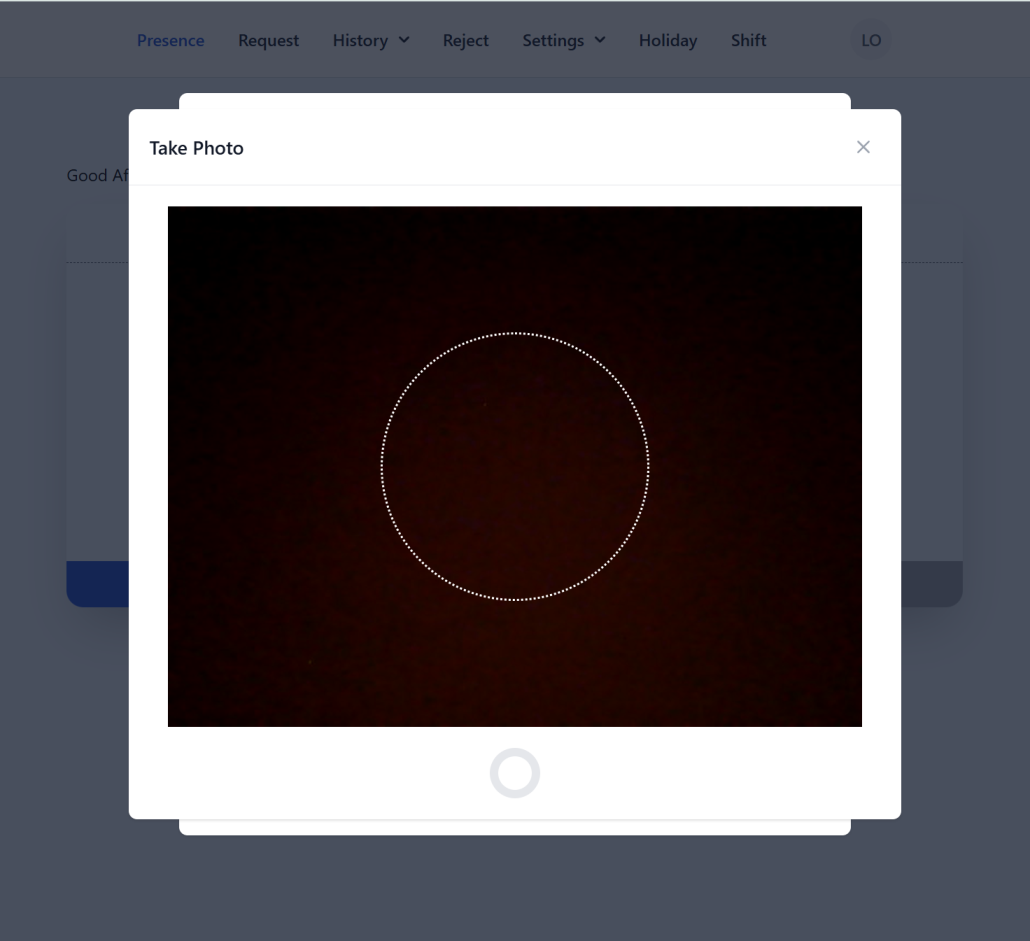
\includegraphics[width=7cm]{Gambar/bab3/modal-kamera-tensorflow.png}
    	\caption{Tampilan Modal Kamera Integrasi TensorFlow}
    	\label{fig:tampilan-kamera-integrasi-tensorflow}
    \end{figure}
    \FloatBarrier
%
%
    \begin{figure}[!htbp]
    	\centering
    	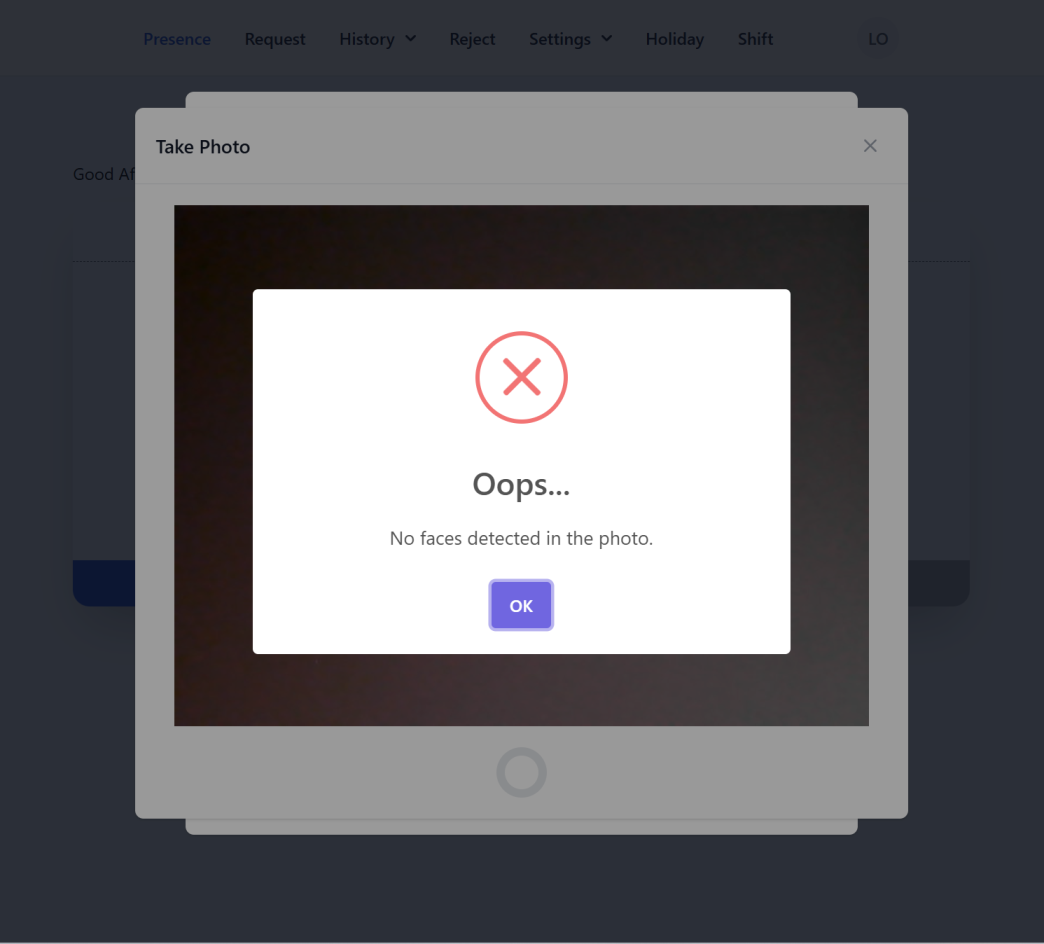
\includegraphics[width=7cm]{Gambar/bab3/no-faces-kamera-tensorflow.png}
    	\caption{Tampilan Validasi \textit{Error} Pengambilan Foto}
    	\label{fig:tampilan-error-validasi-pengambilan-foto}
    \end{figure}
    \FloatBarrier
%
\subsection{Implementasi Perhitungan Lembur Otomatis}
Pada aplikasi presensi \textit{online} akan dilengkapi perhitungan lembur otomatis ketika \textit{Staff Infrastructure} melakukan presensi masuk dan keluar diluar jam kerja \textit{shift} atau pada hari libur perusahaan. Setiap \textit{Staff Infrastructure} akan diatur jenis \textit{shift} yang akan digunakan berdasarkan kurun waktu tertentu. \textbf{\ref{fig:tampilan-pengaturan-jadwal-shift}} menunjukkan halaman modul penjadwalan \textit{shift} yang berisi data nama \textit{staff} "leon ok" akan menggunakan jenis \textit{shift} "password clock" dari tanggal 1 November 2024 hingga 30 November 2024.
 \begin{figure}[!htbp]
    	\centering
    	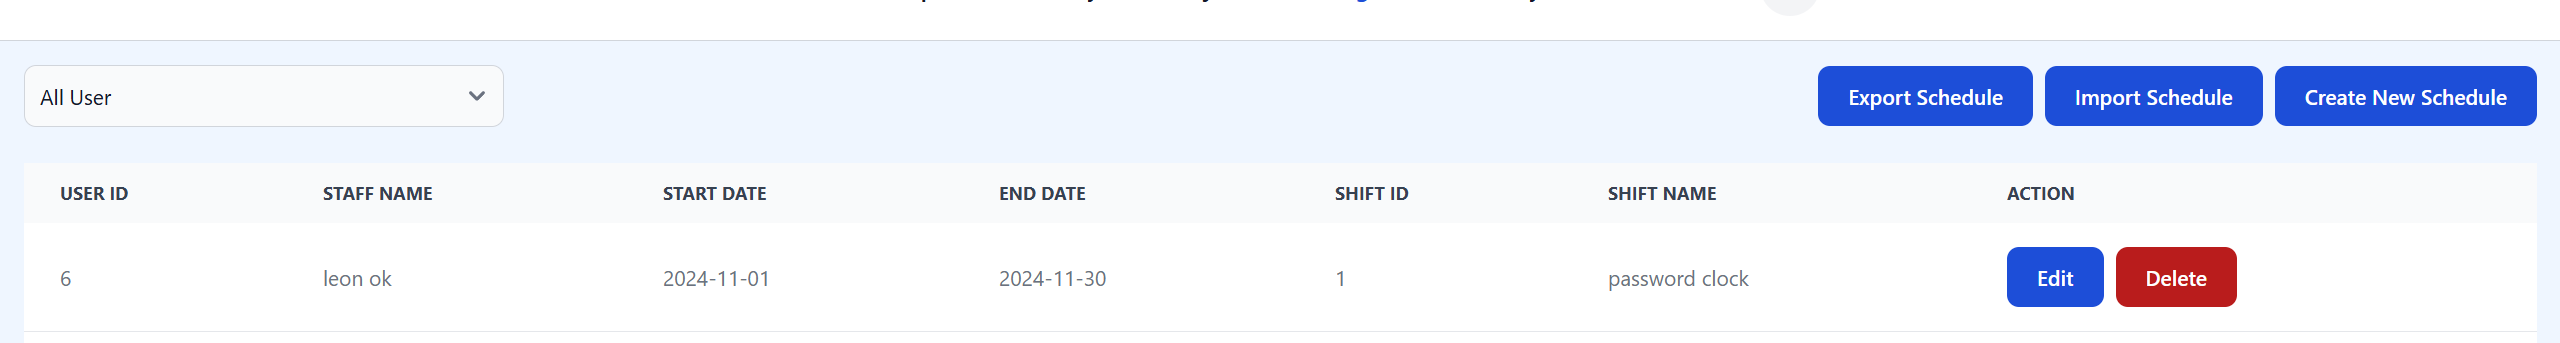
\includegraphics[width=7cm]{Gambar/bab3/implementasi-jadwal-shift.png}
    	\caption{Tampilan Pengaturan Jadwal \textit{Shift}}
    	\label{fig:tampilan-pengaturan-jadwal-shift}
    \end{figure}
    \FloatBarrier
Selanjutnya, masing-masing \textit{Staff Infrastructure} akan diatur jadwal libur yang bisa saja sama antara \textit{staff} satu dengan lainnya maupun sebaliknya. \textbf{\ref{fig:tampilan-pengaturan-libur-staff-infrastructure}} menunjukkan pengaturan jenis libur yang digunakan oleh pengguna.
\begin{figure}[!htbp]
    	\centering
    	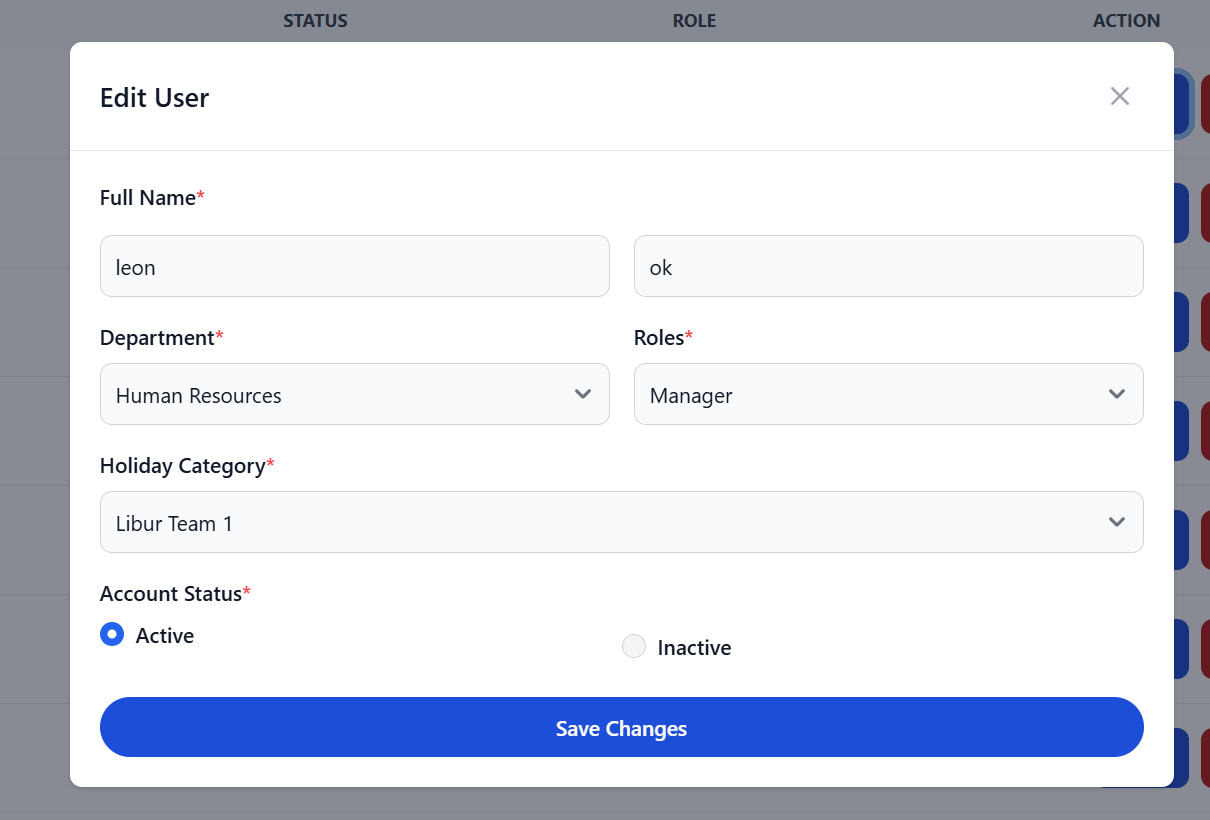
\includegraphics[width=7cm]{Gambar/bab3/implementasi-pengaturan-libur.png}
    	\caption{Tampilan Pengaturan Libur Pada \textit{Staff Infrastructure}}
    	\label{fig:tampilan-pengaturan-libur-staff-infrastructure}
    \end{figure}
    \FloatBarrier

Setelah mengatur penjadwalan \textit{shift} dan libur pada setiap pengguna, maka aplikasi presensi \textit{online} akan otomatis mengecek tanggal dan waktu pengguna setiap melakukan presensi keluar dan membuat data lembur secara otomatis jika presensi dilakukan diluar penjadwalan \textit{shift} yang telah ditentukan ataupun saat hari libur perusahaan. \textbf{\ref{fig:tampilan-lembur-otomatis}} menunjukkan tampilan modal yang memberikan informasi lembur yang dibuat secara otomatis, sistem juga otomatis menghitung total lembur \textit{Staff Infrastructure} dalam satuan menit.
\begin{figure}[!htbp]
    	\centering
    	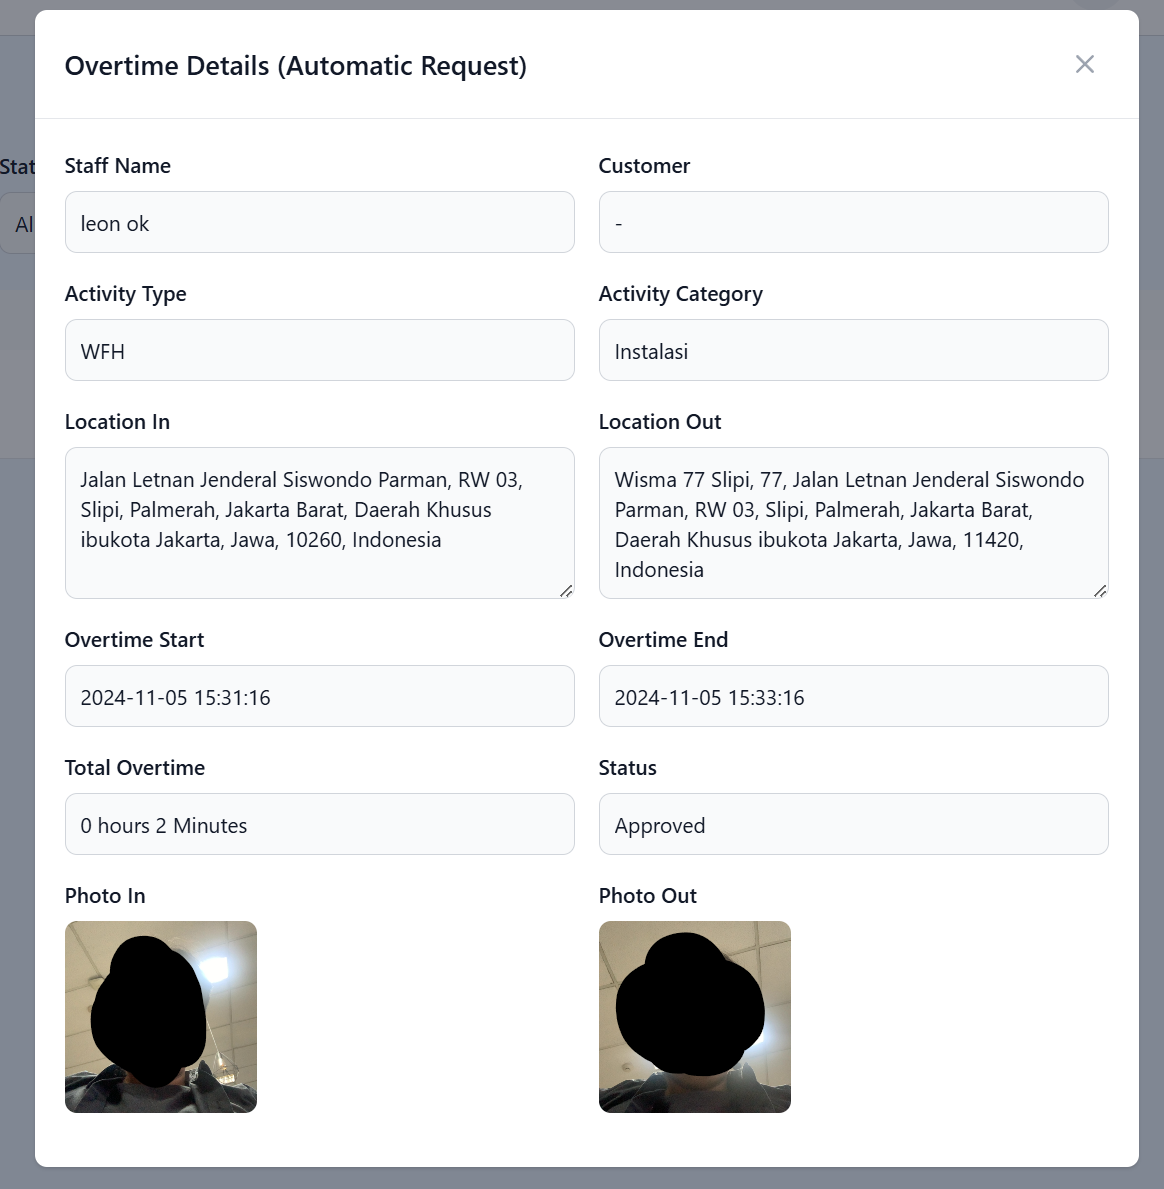
\includegraphics[width=7cm]{Gambar/bab3/implementasi-lembur-otomatis.png}
    	\caption{Tampilan Modal Informasi Lembur Secara Otomatis}
    	\label{fig:tampilan-lembur-otomatis}
    \end{figure}
    \FloatBarrier

\subsection{Implementasi Otorisasi}
Setelah seluruh modul selesai dibuat, maka akan dibuat \textit{middleware} yang berguna untuk membatasi akses modul yang dapat digunakan oleh pengguna. Dalam aplikasi presensi \textit{online} akan terdapat beberapa otorisasi yang digunakan yaitu sebagai berikut:
\begin{enumerate}
    \item \textit{Guest}
    \\ Otorisasi ini berfungsi untuk memberikan akses modul pada pengguna yang belum melakukan autentikasi, seperti modul registrasi dan \textit{login}. 

    \item \textit{Auth}
    \\ Otorisasi ini berfungsi untuk membatasi akses seluruh modul yang mengharuskan pengguna untuk melakukan \textit{authentication} dengan status akun yang telah diverifikasi \textit{email}-nya.
    
    \item \textit{CheckIsActive}
    \\ Otorisasi ini berfungsi untuk mengecek akun pengguna. Jika akun pengguna dengan status \textit{active}, maka dapat mengakses modul sesuai dengan \textit{role} yang diberikan. Jika status \textit{inactive}, maka tidak dapat mengakses seluruh modul dan harus menunggu hingga akun diaktifkan oleh \textit{Manager}.

    \item \textit{CheckSession}
    \\ Otorisasi ini akan mengecek sesi pengguna, jika sebelumnya pengguna sudah melakukan \textit{login} dan kemudian ingin melakukan \textit{login} pada \textit{device} berbeda, maka sesi pada perangkat yang lama akan otomatis ter-\textit{logout}.

    \item \textit{IsManager}
    \\ Otorisasi ini akan membatasi modul yang hanya dapat diakses oleh \textit{role Manager}, seperti \textit{settings department} dan \textit{user}, \textit{shift}, \textit{reject}, dan \textit{holiday}.
\end{enumerate}

\subsection{\textit{Deployment} Aplikasi}
Pada tahap \textit{deployment} aplikasi secara lokal akan menggunakan Artisan CLI yang merupakan salah satu fitur dari Laravel. Cara menjalankan aplikasi dengan server lokal dengan mengetikkan \textit{command line} "php artisan serve". Setelah itu mengatur konfigurasi pada \textit{file} .env yaitu mengubah value APP\_ENV menjadi \textit{local} dan APP\_DEBUG menjadi \textit{true} agar dapat memantau \textit{error} secara langsung. Sedangkan pada \textit{deployment} pada \textit{production} akan menggunakan CPanel. \textit{File project} akan di-\textit{upload} melalui \textit{file manager}. Setelah itu, mengatur \textit{folder public} sebagai \textit{root domain} dan melakukan penyesuaian pada lokasi direktori \textit{folder public} pada \textit{file} autoload.php. Pada \textit{file} .env akan dilakukan konfigurasi berupa APP\_ENV menjadi \textit{production} dan APP\_DEBUG menjadi \textit{false} agar ketika terjadi \textit{error} maka tidak akan memberikan pesan \textit{error} secara detail. Selanjutnya, mengaktifkan SSL untuk keamanan tambahan dikarenakan aplikasi ini memerlukan izin akses lokasi dan kamera pada perangkat.